\documentclass[twoside]{book}

% Packages required by doxygen
\usepackage{fixltx2e}
\usepackage{calc}
\usepackage{doxygen}
\usepackage[export]{adjustbox} % also loads graphicx
\usepackage{graphicx}
\usepackage[utf8]{inputenc}
\usepackage{makeidx}
\usepackage{multicol}
\usepackage{multirow}
\PassOptionsToPackage{warn}{textcomp}
\usepackage{textcomp}
\usepackage[nointegrals]{wasysym}
\usepackage[table]{xcolor}

% Font selection
\usepackage[T1]{fontenc}
\usepackage[scaled=.90]{helvet}
\usepackage{courier}
\usepackage{amssymb}
\usepackage{sectsty}
\renewcommand{\familydefault}{\sfdefault}
\allsectionsfont{%
  \fontseries{bc}\selectfont%
  \color{darkgray}%
}
\renewcommand{\DoxyLabelFont}{%
  \fontseries{bc}\selectfont%
  \color{darkgray}%
}
\newcommand{\+}{\discretionary{\mbox{\scriptsize$\hookleftarrow$}}{}{}}

% Page & text layout
\usepackage{geometry}
\geometry{%
  a4paper,%
  top=2.5cm,%
  bottom=2.5cm,%
  left=2.5cm,%
  right=2.5cm%
}
\tolerance=750
\hfuzz=15pt
\hbadness=750
\setlength{\emergencystretch}{15pt}
\setlength{\parindent}{0cm}
\setlength{\parskip}{3ex plus 2ex minus 2ex}
\makeatletter
\renewcommand{\paragraph}{%
  \@startsection{paragraph}{4}{0ex}{-1.0ex}{1.0ex}{%
    \normalfont\normalsize\bfseries\SS@parafont%
  }%
}
\renewcommand{\subparagraph}{%
  \@startsection{subparagraph}{5}{0ex}{-1.0ex}{1.0ex}{%
    \normalfont\normalsize\bfseries\SS@subparafont%
  }%
}
\makeatother

% Headers & footers
\usepackage{fancyhdr}
\pagestyle{fancyplain}
\fancyhead[LE]{\fancyplain{}{\bfseries\thepage}}
\fancyhead[CE]{\fancyplain{}{}}
\fancyhead[RE]{\fancyplain{}{\bfseries\leftmark}}
\fancyhead[LO]{\fancyplain{}{\bfseries\rightmark}}
\fancyhead[CO]{\fancyplain{}{}}
\fancyhead[RO]{\fancyplain{}{\bfseries\thepage}}
\fancyfoot[LE]{\fancyplain{}{}}
\fancyfoot[CE]{\fancyplain{}{}}
\fancyfoot[RE]{\fancyplain{}{\bfseries\scriptsize Generated by Doxygen }}
\fancyfoot[LO]{\fancyplain{}{\bfseries\scriptsize Generated by Doxygen }}
\fancyfoot[CO]{\fancyplain{}{}}
\fancyfoot[RO]{\fancyplain{}{}}
\renewcommand{\footrulewidth}{0.4pt}
\renewcommand{\chaptermark}[1]{%
  \markboth{#1}{}%
}
\renewcommand{\sectionmark}[1]{%
  \markright{\thesection\ #1}%
}

% Indices & bibliography
\usepackage{natbib}
\usepackage[titles]{tocloft}
\setcounter{tocdepth}{3}
\setcounter{secnumdepth}{5}
\makeindex

% Hyperlinks (required, but should be loaded last)
\usepackage{ifpdf}
\ifpdf
  \usepackage[pdftex,pagebackref=true]{hyperref}
\else
  \usepackage[ps2pdf,pagebackref=true]{hyperref}
\fi
\hypersetup{%
  colorlinks=true,%
  linkcolor=blue,%
  citecolor=blue,%
  unicode%
}

% Custom commands
\newcommand{\clearemptydoublepage}{%
  \newpage{\pagestyle{empty}\cleardoublepage}%
}

\usepackage{caption}
\captionsetup{labelsep=space,justification=centering,font={bf},singlelinecheck=off,skip=4pt,position=top}

%===== C O N T E N T S =====

\begin{document}

% Titlepage & ToC
\hypersetup{pageanchor=false,
             bookmarksnumbered=true,
             pdfencoding=unicode
            }
\pagenumbering{roman}
\begin{titlepage}
\vspace*{7cm}
\begin{center}%
{\Large My Project }\\
\vspace*{1cm}
{\large Generated by Doxygen 1.8.11}\\
\end{center}
\end{titlepage}
\clearemptydoublepage
\tableofcontents
\clearemptydoublepage
\pagenumbering{arabic}
\hypersetup{pageanchor=true}

%--- Begin generated contents ---
\chapter{Data Structure Index}
\section{Data Structures}
Here are the data structures with brief descriptions\+:\begin{DoxyCompactList}
\item\contentsline{section}{\hyperlink{structbackground}{background} }{\pageref{structbackground}}{}
\item\contentsline{section}{\hyperlink{structenemy}{enemy} \\*Struct for backround }{\pageref{structenemy}}{}
\item\contentsline{section}{\hyperlink{structenigme}{enigme} }{\pageref{structenigme}}{}
\item\contentsline{section}{\hyperlink{structminimap}{minimap} \\*Struct for backround }{\pageref{structminimap}}{}
\item\contentsline{section}{\hyperlink{structPersonne}{Personne} \\*Struct for perso }{\pageref{structPersonne}}{}
\item\contentsline{section}{\hyperlink{structtext}{text} }{\pageref{structtext}}{}
\item\contentsline{section}{\hyperlink{structtime}{time} }{\pageref{structtime}}{}
\end{DoxyCompactList}

\chapter{File Index}
\section{File List}
Here is a list of all documented files with brief descriptions\+:\begin{DoxyCompactList}
\item\contentsline{section}{\hyperlink{background_8c}{background.\+c} }{\pageref{background_8c}}{}
\item\contentsline{section}{{\bfseries background.\+h} }{\pageref{background_8h}}{}
\item\contentsline{section}{\hyperlink{enemy_8c}{enemy.\+c} }{\pageref{enemy_8c}}{}
\item\contentsline{section}{{\bfseries enemy.\+h} }{\pageref{enemy_8h}}{}
\item\contentsline{section}{\hyperlink{enigme_8c}{enigme.\+c} }{\pageref{enigme_8c}}{}
\item\contentsline{section}{{\bfseries enigme.\+h} }{\pageref{enigme_8h}}{}
\item\contentsline{section}{\hyperlink{enigmealeatoire_8c}{enigmealeatoire.\+c} }{\pageref{enigmealeatoire_8c}}{}
\item\contentsline{section}{{\bfseries enigmealeatoire.\+h} }{\pageref{enigmealeatoire_8h}}{}
\item\contentsline{section}{\hyperlink{main_8c}{main.\+c} \\*Testing Program }{\pageref{main_8c}}{}
\item\contentsline{section}{{\bfseries main.\+h} }{\pageref{main_8h}}{}
\item\contentsline{section}{\hyperlink{minimap_8c}{minimap.\+c} }{\pageref{minimap_8c}}{}
\item\contentsline{section}{{\bfseries minimap.\+h} }{\pageref{minimap_8h}}{}
\item\contentsline{section}{\hyperlink{perso_8c}{perso.\+c} }{\pageref{perso_8c}}{}
\item\contentsline{section}{{\bfseries perso.\+h} }{\pageref{perso_8h}}{}
\item\contentsline{section}{\hyperlink{save_8c}{save.\+c} }{\pageref{save_8c}}{}
\item\contentsline{section}{{\bfseries save.\+h} }{\pageref{save_8h}}{}
\item\contentsline{section}{{\bfseries lot1/type.\+h} }{\pageref{lot1_2type_8h}}{}
\item\contentsline{section}{{\bfseries lot2/type.\+h} }{\pageref{lot2_2type_8h}}{}
\item\contentsline{section}{{\bfseries lot3/type.\+h} }{\pageref{lot3_2type_8h}}{}
\item\contentsline{section}{{\bfseries lot4/type.\+h} }{\pageref{lot4_2type_8h}}{}
\item\contentsline{section}{{\bfseries lot5/type.\+h} }{\pageref{lot5_2type_8h}}{}
\item\contentsline{section}{{\bfseries lot6/type.\+h} }{\pageref{lot6_2type_8h}}{}
\item\contentsline{section}{{\bfseries lot7/type.\+h} }{\pageref{lot7_2type_8h}}{}
\end{DoxyCompactList}

\chapter{Data Structure Documentation}
\hypertarget{structbackground}{}\section{background Struct Reference}
\label{structbackground}\index{background@{background}}
\subsection*{Data Fields}
\begin{DoxyCompactItemize}
\item 
S\+D\+L\+\_\+\+Surface $\ast$ {\bfseries image}\hypertarget{structbackground_a321e7102a3c80e33d40a276f09b8e3f6}{}\label{structbackground_a321e7102a3c80e33d40a276f09b8e3f6}

\item 
S\+D\+L\+\_\+\+Surface $\ast$ {\bfseries image1}\hypertarget{structbackground_a383993cef3e7438fbd6b11f1b2b40b3b}{}\label{structbackground_a383993cef3e7438fbd6b11f1b2b40b3b}

\item 
S\+D\+L\+\_\+\+Surface $\ast$ {\bfseries checkpoint1}\hypertarget{structbackground_a85541518908a04c627087ad7aaf52b0f}{}\label{structbackground_a85541518908a04c627087ad7aaf52b0f}

\item 
S\+D\+L\+\_\+\+Rect {\bfseries cp1}\hypertarget{structbackground_acd1460099638e81dc1dbcff38db97ade}{}\label{structbackground_acd1460099638e81dc1dbcff38db97ade}

\item 
S\+D\+L\+\_\+\+Surface $\ast$ {\bfseries checkpoint2}\hypertarget{structbackground_a21365a26147b3d4e257eef58ed368082}{}\label{structbackground_a21365a26147b3d4e257eef58ed368082}

\item 
S\+D\+L\+\_\+\+Rect {\bfseries cp2}\hypertarget{structbackground_ab79b3c0a246650c2f5cd7c6613edcb13}{}\label{structbackground_ab79b3c0a246650c2f5cd7c6613edcb13}

\item 
S\+D\+L\+\_\+\+Surface $\ast$ {\bfseries traps}\hypertarget{structbackground_aaa1e151b245173a5e77f6a3a3a5c37ef}{}\label{structbackground_aaa1e151b245173a5e77f6a3a3a5c37ef}

\item 
S\+D\+L\+\_\+\+Surface $\ast$ {\bfseries win}\hypertarget{structbackground_ab61ca008f371cdf1ba9f8e80238df001}{}\label{structbackground_ab61ca008f371cdf1ba9f8e80238df001}

\item 
S\+D\+L\+\_\+\+Surface $\ast$ {\bfseries menu}\hypertarget{structbackground_a13494e2a1274aef0579ac884e7d97973}{}\label{structbackground_a13494e2a1274aef0579ac884e7d97973}

\item 
S\+D\+L\+\_\+\+Surface $\ast$ {\bfseries save}\hypertarget{structbackground_a0b562c57eaa92a2f663bbded09349bf3}{}\label{structbackground_a0b562c57eaa92a2f663bbded09349bf3}

\item 
S\+D\+L\+\_\+\+Surface $\ast$ {\bfseries load}\hypertarget{structbackground_ae3171998bc7d421d66997de00772f05f}{}\label{structbackground_ae3171998bc7d421d66997de00772f05f}

\item 
S\+D\+L\+\_\+\+Surface $\ast$ {\bfseries exit}\hypertarget{structbackground_acfd06863a42d3ad13e229cdc33042001}{}\label{structbackground_acfd06863a42d3ad13e229cdc33042001}

\item 
S\+D\+L\+\_\+\+Surface $\ast$ {\bfseries newgame}\hypertarget{structbackground_acca5f15fc1db8659f1f43a17e3e6dba7}{}\label{structbackground_acca5f15fc1db8659f1f43a17e3e6dba7}

\item 
S\+D\+L\+\_\+\+Rect {\bfseries position\+Ecran}\hypertarget{structbackground_ac49e9f0e97cbb8e4088edab9fcaf6b52}{}\label{structbackground_ac49e9f0e97cbb8e4088edab9fcaf6b52}

\item 
S\+D\+L\+\_\+\+Rect {\bfseries Camera}\hypertarget{structbackground_a267b1d8afe86ab79bd9069c079137468}{}\label{structbackground_a267b1d8afe86ab79bd9069c079137468}

\item 
S\+D\+L\+\_\+\+Rect {\bfseries trapsP}\hypertarget{structbackground_a2210d12272e0361502a107db5d6340f4}{}\label{structbackground_a2210d12272e0361502a107db5d6340f4}

\item 
S\+D\+L\+\_\+\+Rect {\bfseries winP}\hypertarget{structbackground_aa0146875963fceb97109683f93422758}{}\label{structbackground_aa0146875963fceb97109683f93422758}

\item 
S\+D\+L\+\_\+\+Rect {\bfseries menuP}\hypertarget{structbackground_a189056a0a24b845d3186664e098f422a}{}\label{structbackground_a189056a0a24b845d3186664e098f422a}

\item 
S\+D\+L\+\_\+\+Rect {\bfseries saveP}\hypertarget{structbackground_af8f5ac164c059bc21f4e822d77309353}{}\label{structbackground_af8f5ac164c059bc21f4e822d77309353}

\item 
S\+D\+L\+\_\+\+Rect {\bfseries loadP}\hypertarget{structbackground_ad1fab57d015a9770bf50f5e3d38089e6}{}\label{structbackground_ad1fab57d015a9770bf50f5e3d38089e6}

\item 
S\+D\+L\+\_\+\+Rect {\bfseries exitP}\hypertarget{structbackground_a2360abe185abdf12fd8583bfd70f66ae}{}\label{structbackground_a2360abe185abdf12fd8583bfd70f66ae}

\item 
S\+D\+L\+\_\+\+Rect {\bfseries newgameP}\hypertarget{structbackground_a5476a37aac815215b2e66b31852a337c}{}\label{structbackground_a5476a37aac815215b2e66b31852a337c}

\end{DoxyCompactItemize}


The documentation for this struct was generated from the following file\+:\begin{DoxyCompactItemize}
\item 
lot3/type.\+h\end{DoxyCompactItemize}

\hypertarget{structenemy}{}\section{enemy Struct Reference}
\label{structenemy}\index{enemy@{enemy}}


struct for backround  




{\ttfamily \#include \char`\"{}type.\+h\char`\"{}}

\subsection*{Data Fields}
\begin{DoxyCompactItemize}
\item 
S\+D\+L\+\_\+\+Surface $\ast$ {\bfseries image1}\hypertarget{structenemy_a95d99f3c8c142987c1667b352aff9645}{}\label{structenemy_a95d99f3c8c142987c1667b352aff9645}

\item 
S\+D\+L\+\_\+\+Surface $\ast$ {\bfseries image2}\hypertarget{structenemy_a9da85313d408136c35fb512e4b6a3c9c}{}\label{structenemy_a9da85313d408136c35fb512e4b6a3c9c}

\item 
S\+D\+L\+\_\+\+Surface $\ast$ {\bfseries image3}\hypertarget{structenemy_a326c9d9097a4126c0352a133b66cad79}{}\label{structenemy_a326c9d9097a4126c0352a133b66cad79}

\item 
S\+D\+L\+\_\+\+Surface $\ast$ {\bfseries image4}\hypertarget{structenemy_ab2a6c3af7dcda7a12b9e5214fcb9424c}{}\label{structenemy_ab2a6c3af7dcda7a12b9e5214fcb9424c}

\item 
S\+D\+L\+\_\+\+Surface $\ast$ {\bfseries image\+Enemy\+Avant} \mbox{[}3\mbox{]}\mbox{[}2\mbox{]}\hypertarget{structenemy_a06ee8a6870059b8eb9e69cd012e67fcb}{}\label{structenemy_a06ee8a6870059b8eb9e69cd012e67fcb}

\item 
S\+D\+L\+\_\+\+Rect {\bfseries position\+Ecran\+Enemy}\hypertarget{structenemy_ae89081bba474c910c1964fed335f6e06}{}\label{structenemy_ae89081bba474c910c1964fed335f6e06}

\item 
int {\bfseries direction}\hypertarget{structenemy_a6c1787380ba9a394339941a8e41a8737}{}\label{structenemy_a6c1787380ba9a394339941a8e41a8737}

\end{DoxyCompactItemize}


\subsection{Detailed Description}
struct for backround 

The documentation for this struct was generated from the following file\+:\begin{DoxyCompactItemize}
\item 
lot2/type.\+h\end{DoxyCompactItemize}

\hypertarget{structenigme}{}\section{enigme Struct Reference}
\label{structenigme}\index{enigme@{enigme}}
\subsection*{Data Fields}
\begin{DoxyCompactItemize}
\item 
char {\bfseries question} \mbox{[}200\mbox{]}\hypertarget{structenigme_a13c263b6a2a06090e3b87ca725152ffb}{}\label{structenigme_a13c263b6a2a06090e3b87ca725152ffb}

\item 
char {\bfseries reponse1} \mbox{[}200\mbox{]}\hypertarget{structenigme_a1d31bead9270c4be04f410820b285ade}{}\label{structenigme_a1d31bead9270c4be04f410820b285ade}

\item 
char {\bfseries reponse2} \mbox{[}200\mbox{]}\hypertarget{structenigme_a97f9390bd04fc83a0a7a84f3bf03464d}{}\label{structenigme_a97f9390bd04fc83a0a7a84f3bf03464d}

\item 
char {\bfseries reponse3} \mbox{[}200\mbox{]}\hypertarget{structenigme_ad7f3c27ab2d1e20502ee3a39040c99f3}{}\label{structenigme_ad7f3c27ab2d1e20502ee3a39040c99f3}

\item 
S\+D\+L\+\_\+\+Surface $\ast$ {\bfseries img}\hypertarget{structenigme_ac5c2141e5f8c366ff16d1fad83ee3e54}{}\label{structenigme_ac5c2141e5f8c366ff16d1fad83ee3e54}

\item 
int {\bfseries numrepjuste}\hypertarget{structenigme_a0d5d54cb6600ef161c4bcb717056432e}{}\label{structenigme_a0d5d54cb6600ef161c4bcb717056432e}

\item 
T\+T\+F\+\_\+\+Font $\ast$ {\bfseries police}\hypertarget{structenigme_a63ffe54c589cabf303d7240afec104e5}{}\label{structenigme_a63ffe54c589cabf303d7240afec104e5}

\item 
T\+T\+F\+\_\+\+Font $\ast$ {\bfseries policequestion}\hypertarget{structenigme_a777fe6d777b296ad91d09a8473f6b1ca}{}\label{structenigme_a777fe6d777b296ad91d09a8473f6b1ca}

\item 
S\+D\+L\+\_\+\+Surface $\ast$ {\bfseries textequestion}\hypertarget{structenigme_a2028fcc3934ef8042304fb68fcc848c5}{}\label{structenigme_a2028fcc3934ef8042304fb68fcc848c5}

\item 
S\+D\+L\+\_\+\+Surface $\ast$ {\bfseries texterep1}\hypertarget{structenigme_a23dab2ed05449faefdd9063173770ccd}{}\label{structenigme_a23dab2ed05449faefdd9063173770ccd}

\item 
S\+D\+L\+\_\+\+Surface $\ast$ {\bfseries texterep2}\hypertarget{structenigme_ac36028b78e018d3c4add8202ecd0a764}{}\label{structenigme_ac36028b78e018d3c4add8202ecd0a764}

\item 
S\+D\+L\+\_\+\+Surface $\ast$ {\bfseries texterep3}\hypertarget{structenigme_a345316bb9abe878261190f089d71c602}{}\label{structenigme_a345316bb9abe878261190f089d71c602}

\item 
S\+D\+L\+\_\+\+Rect {\bfseries posquestion}\hypertarget{structenigme_a8aadd5abb9637ce335e809eb38d71c1b}{}\label{structenigme_a8aadd5abb9637ce335e809eb38d71c1b}

\item 
S\+D\+L\+\_\+\+Rect {\bfseries posreponse1}\hypertarget{structenigme_af3cd0f8dd54fa350fc40afbfdac8fb0a}{}\label{structenigme_af3cd0f8dd54fa350fc40afbfdac8fb0a}

\item 
S\+D\+L\+\_\+\+Rect {\bfseries posreponse2}\hypertarget{structenigme_a24dc6a7818358bf6b0ce5fd88c93b8d0}{}\label{structenigme_a24dc6a7818358bf6b0ce5fd88c93b8d0}

\item 
S\+D\+L\+\_\+\+Rect {\bfseries posreponse3}\hypertarget{structenigme_ad631d08560c027e35a586af9e093ca32}{}\label{structenigme_ad631d08560c027e35a586af9e093ca32}

\item 
S\+D\+L\+\_\+\+Rect {\bfseries posimg}\hypertarget{structenigme_ae7a374c2aadba6ed543d8cc47705d141}{}\label{structenigme_ae7a374c2aadba6ed543d8cc47705d141}

\item 
S\+D\+L\+\_\+\+Rect {\bfseries posboard}\hypertarget{structenigme_ac374f2148e8955fcf0a82b475e13c1d6}{}\label{structenigme_ac374f2148e8955fcf0a82b475e13c1d6}

\item 
S\+D\+L\+\_\+\+Surface $\ast$ {\bfseries imgboard}\hypertarget{structenigme_a5a9d93cf486be4b5cb5003a007694701}{}\label{structenigme_a5a9d93cf486be4b5cb5003a007694701}

\item 
S\+D\+L\+\_\+\+Rect {\bfseries posbravo}\hypertarget{structenigme_a4df3124b326cdfc7cc5fc37984fa9da9}{}\label{structenigme_a4df3124b326cdfc7cc5fc37984fa9da9}

\item 
S\+D\+L\+\_\+\+Surface $\ast$ {\bfseries textebravo}\hypertarget{structenigme_a09b53fa41d97fb5cb9a970798428258f}{}\label{structenigme_a09b53fa41d97fb5cb9a970798428258f}

\item 
T\+T\+F\+\_\+\+Font $\ast$ {\bfseries policebravo}\hypertarget{structenigme_abf756a2f29a81805e5b56d90366dc6ce}{}\label{structenigme_abf756a2f29a81805e5b56d90366dc6ce}

\item 
S\+D\+L\+\_\+\+Rect {\bfseries posincorrecte}\hypertarget{structenigme_a0d0604efc06bac24975ff24623e8b547}{}\label{structenigme_a0d0604efc06bac24975ff24623e8b547}

\item 
T\+T\+F\+\_\+\+Font $\ast$ {\bfseries policeincorrecte}\hypertarget{structenigme_af37fcd4fa7190184d2b8e06ab031a471}{}\label{structenigme_af37fcd4fa7190184d2b8e06ab031a471}

\item 
S\+D\+L\+\_\+\+Surface $\ast$ {\bfseries texteincorrecte}\hypertarget{structenigme_a4c20af04bbfb38fc9c528a8d89bcc2d8}{}\label{structenigme_a4c20af04bbfb38fc9c528a8d89bcc2d8}

\end{DoxyCompactItemize}


The documentation for this struct was generated from the following file\+:\begin{DoxyCompactItemize}
\item 
lot6/type.\+h\end{DoxyCompactItemize}

\hypertarget{structminimap}{}\section{minimap Struct Reference}
\label{structminimap}\index{minimap@{minimap}}


struct for backround  




{\ttfamily \#include \char`\"{}type.\+h\char`\"{}}

\subsection*{Data Fields}
\begin{DoxyCompactItemize}
\item 
S\+D\+L\+\_\+\+Surface $\ast$ {\bfseries image\+De\+Fond}\hypertarget{structminimap_a4209795915394333a274ce236431312e}{}\label{structminimap_a4209795915394333a274ce236431312e}

\item 
S\+D\+L\+\_\+\+Rect {\bfseries position\+Fond}\hypertarget{structminimap_a2f529aabfdb3b15e5991ea91ca48aaa6}{}\label{structminimap_a2f529aabfdb3b15e5991ea91ca48aaa6}

\item 
S\+D\+L\+\_\+\+Surface $\ast$ {\bfseries detective}\hypertarget{structminimap_a850de5a08feed651a4fa63ef64256708}{}\label{structminimap_a850de5a08feed651a4fa63ef64256708}

\item 
S\+D\+L\+\_\+\+Rect {\bfseries positiondetective}\hypertarget{structminimap_a9466c88ff7ccadf25b23590be92813be}{}\label{structminimap_a9466c88ff7ccadf25b23590be92813be}

\end{DoxyCompactItemize}


\subsection{Detailed Description}
struct for backround 

The documentation for this struct was generated from the following file\+:\begin{DoxyCompactItemize}
\item 
lot4/type.\+h\end{DoxyCompactItemize}

\hypertarget{structPersonne}{}\section{Personne Struct Reference}
\label{structPersonne}\index{Personne@{Personne}}


struct for perso  




{\ttfamily \#include \char`\"{}type.\+h\char`\"{}}

\subsection*{Data Fields}
\begin{DoxyCompactItemize}
\item 
S\+D\+L\+\_\+\+Surface $\ast$ {\bfseries image1}\hypertarget{structPersonne_a5ba6ae4971a61519fb5fb44c27416ba2}{}\label{structPersonne_a5ba6ae4971a61519fb5fb44c27416ba2}

\item 
S\+D\+L\+\_\+\+Surface $\ast$ {\bfseries image2}\hypertarget{structPersonne_abdb0a6b3b6f077d2ac6d93bce38950bd}{}\label{structPersonne_abdb0a6b3b6f077d2ac6d93bce38950bd}

\item 
S\+D\+L\+\_\+\+Surface $\ast$ {\bfseries image3}\hypertarget{structPersonne_a018b17557fcf0d8d21f6b24be4b1fa75}{}\label{structPersonne_a018b17557fcf0d8d21f6b24be4b1fa75}

\item 
S\+D\+L\+\_\+\+Surface $\ast$ {\bfseries image4}\hypertarget{structPersonne_a96d7128e0af43f1ee20893ebe7ec81d5}{}\label{structPersonne_a96d7128e0af43f1ee20893ebe7ec81d5}

\item 
S\+D\+L\+\_\+\+Surface $\ast$ {\bfseries image5}\hypertarget{structPersonne_a79f12b68dbbd5890d2178a94e6656d39}{}\label{structPersonne_a79f12b68dbbd5890d2178a94e6656d39}

\item 
S\+D\+L\+\_\+\+Surface $\ast$ {\bfseries image6}\hypertarget{structPersonne_aae809af7db85d2a70dcb486a2fe67368}{}\label{structPersonne_aae809af7db85d2a70dcb486a2fe67368}

\item 
S\+D\+L\+\_\+\+Surface $\ast$ {\bfseries image7}\hypertarget{structPersonne_ae9ae7943f9a0575983302f5bf26a5b5a}{}\label{structPersonne_ae9ae7943f9a0575983302f5bf26a5b5a}

\item 
S\+D\+L\+\_\+\+Surface $\ast$ {\bfseries image8}\hypertarget{structPersonne_abf531adac765ed47acef036040ed929a}{}\label{structPersonne_abf531adac765ed47acef036040ed929a}

\item 
S\+D\+L\+\_\+\+Surface $\ast$ {\bfseries image9}\hypertarget{structPersonne_a1f0c6aa603ef91e1c7fbe699691b96fc}{}\label{structPersonne_a1f0c6aa603ef91e1c7fbe699691b96fc}

\item 
S\+D\+L\+\_\+\+Surface $\ast$ {\bfseries image10}\hypertarget{structPersonne_a0af0082b7015ffe7b50b6ae0f7092443}{}\label{structPersonne_a0af0082b7015ffe7b50b6ae0f7092443}

\item 
S\+D\+L\+\_\+\+Surface $\ast$ {\bfseries image11}\hypertarget{structPersonne_a2e38bb031b6612501c5cdb975026746d}{}\label{structPersonne_a2e38bb031b6612501c5cdb975026746d}

\item 
S\+D\+L\+\_\+\+Surface $\ast$ {\bfseries image12}\hypertarget{structPersonne_a43e16a70610f1b8d47825714167a2f66}{}\label{structPersonne_a43e16a70610f1b8d47825714167a2f66}

\item 
S\+D\+L\+\_\+\+Surface $\ast$ {\bfseries image13}\hypertarget{structPersonne_a1a2f315ab8c30fcbffcebf110d7c7906}{}\label{structPersonne_a1a2f315ab8c30fcbffcebf110d7c7906}

\item 
S\+D\+L\+\_\+\+Surface $\ast$ {\bfseries imageperso\+Avant} \mbox{[}7\mbox{]}\mbox{[}5\mbox{]}\hypertarget{structPersonne_a24eb0c11c2b148042d9c3b99edcdff78}{}\label{structPersonne_a24eb0c11c2b148042d9c3b99edcdff78}

\item 
S\+D\+L\+\_\+\+Rect {\bfseries position\+Ecran\+Perso}\hypertarget{structPersonne_a9b5a3033b6711f5a2a1f988c65473b73}{}\label{structPersonne_a9b5a3033b6711f5a2a1f988c65473b73}

\item 
S\+D\+L\+\_\+\+Rect {\bfseries position\+Ecran\+Death}\hypertarget{structPersonne_ab5332bbd27448198d831a9a00aa473e2}{}\label{structPersonne_ab5332bbd27448198d831a9a00aa473e2}

\item 
S\+D\+L\+\_\+\+Rect {\bfseries ult}\hypertarget{structPersonne_abf3f6484d187990b2230e12ed19dcafe}{}\label{structPersonne_abf3f6484d187990b2230e12ed19dcafe}

\item 
S\+D\+L\+\_\+\+Surface $\ast$ {\bfseries score}\hypertarget{structPersonne_a25fd98485efb9096da557c9a03934eaf}{}\label{structPersonne_a25fd98485efb9096da557c9a03934eaf}

\item 
S\+D\+L\+\_\+\+Rect {\bfseries position\+Ecran\+Score}\hypertarget{structPersonne_ad9756a3349094bb34a65ed714b393de7}{}\label{structPersonne_ad9756a3349094bb34a65ed714b393de7}

\item 
S\+D\+L\+\_\+\+Surface $\ast$ {\bfseries image000}\hypertarget{structPersonne_a64e121fcdf44d3a2f302c1430190bbb4}{}\label{structPersonne_a64e121fcdf44d3a2f302c1430190bbb4}

\item 
S\+D\+L\+\_\+\+Surface $\ast$ {\bfseries image111}\hypertarget{structPersonne_a9856cf1503a537de14e853a41891d41d}{}\label{structPersonne_a9856cf1503a537de14e853a41891d41d}

\item 
S\+D\+L\+\_\+\+Surface $\ast$ {\bfseries image222}\hypertarget{structPersonne_a0f28b2d9e420b780d4e632aa6d32495f}{}\label{structPersonne_a0f28b2d9e420b780d4e632aa6d32495f}

\item 
S\+D\+L\+\_\+\+Surface $\ast$ {\bfseries image333}\hypertarget{structPersonne_a14f5303fe371dcd407bb33405e3e7bbb}{}\label{structPersonne_a14f5303fe371dcd407bb33405e3e7bbb}

\item 
S\+D\+L\+\_\+\+Surface $\ast$ {\bfseries image444}\hypertarget{structPersonne_acc6c1d4b37a41df75a1128ff4a846541}{}\label{structPersonne_acc6c1d4b37a41df75a1128ff4a846541}

\item 
S\+D\+L\+\_\+\+Surface $\ast$ {\bfseries image555}\hypertarget{structPersonne_a76df67c1f88ccab197794fb24fa1d3f2}{}\label{structPersonne_a76df67c1f88ccab197794fb24fa1d3f2}

\item 
S\+D\+L\+\_\+\+Surface $\ast$ {\bfseries vie} \mbox{[}6\mbox{]}\hypertarget{structPersonne_a9f2945c73bf1d638375d0da1c47f9c8e}{}\label{structPersonne_a9f2945c73bf1d638375d0da1c47f9c8e}

\item 
S\+D\+L\+\_\+\+Rect {\bfseries position\+Ecran\+Vie}\hypertarget{structPersonne_a5a4f0db4e35f43a54e37330504e8da75}{}\label{structPersonne_a5a4f0db4e35f43a54e37330504e8da75}

\item 
double {\bfseries vitesse}\hypertarget{structPersonne_a5f3b440f1baea5a03e7b76d3f27b773a}{}\label{structPersonne_a5f3b440f1baea5a03e7b76d3f27b773a}

\item 
double {\bfseries acceleration}\hypertarget{structPersonne_ac757341de95d4d2b1aa30075aa8df51b}{}\label{structPersonne_ac757341de95d4d2b1aa30075aa8df51b}

\item 
S\+D\+L\+\_\+\+Surface $\ast$ {\bfseries end}\hypertarget{structPersonne_af24e28d8faaeed2bedb23f5e7b038207}{}\label{structPersonne_af24e28d8faaeed2bedb23f5e7b038207}

\item 
S\+D\+L\+\_\+\+Rect {\bfseries position\+Ecran\+End}\hypertarget{structPersonne_ab5d29c733617e93f847df8a19251262e}{}\label{structPersonne_ab5d29c733617e93f847df8a19251262e}

\end{DoxyCompactItemize}


\subsection{Detailed Description}
struct for perso 

The documentation for this struct was generated from the following file\+:\begin{DoxyCompactItemize}
\item 
lot1/type.\+h\end{DoxyCompactItemize}

\hypertarget{structtext}{}\section{text Struct Reference}
\label{structtext}\index{text@{text}}
\subsection*{Data Fields}
\begin{DoxyCompactItemize}
\item 
S\+D\+L\+\_\+\+Surface $\ast$ \hyperlink{structtext_a1a9992f493ebd8946dc5a736d65e8213}{text\+Surface}
\item 
S\+D\+L\+\_\+\+Rect \hyperlink{structtext_a01cc24369eccbe9ccb68af9a748315d3}{position\+Text}
\item 
char {\bfseries txt} \mbox{[}20\mbox{]}\hypertarget{structtext_afd7610607c0ade6ed450f86e275ddce5}{}\label{structtext_afd7610607c0ade6ed450f86e275ddce5}

\item 
S\+D\+L\+\_\+\+Color {\bfseries couleur\+Txt}\hypertarget{structtext_a0f3134d4dbc64c9b28fa625fb627f9c5}{}\label{structtext_a0f3134d4dbc64c9b28fa625fb627f9c5}

\item 
T\+T\+F\+\_\+\+Font $\ast$ {\bfseries police}\hypertarget{structtext_aec9ba02a1c093b1db8aa0f16ac092459}{}\label{structtext_aec9ba02a1c093b1db8aa0f16ac092459}

\end{DoxyCompactItemize}


\subsection{Field Documentation}
\index{text@{text}!position\+Text@{position\+Text}}
\index{position\+Text@{position\+Text}!text@{text}}
\subsubsection[{\texorpdfstring{position\+Text}{positionText}}]{\setlength{\rightskip}{0pt plus 5cm}S\+D\+L\+\_\+\+Rect text\+::position\+Text}\hypertarget{structtext_a01cc24369eccbe9ccb68af9a748315d3}{}\label{structtext_a01cc24369eccbe9ccb68af9a748315d3}
Rectangle \index{text@{text}!text\+Surface@{text\+Surface}}
\index{text\+Surface@{text\+Surface}!text@{text}}
\subsubsection[{\texorpdfstring{text\+Surface}{textSurface}}]{\setlength{\rightskip}{0pt plus 5cm}S\+D\+L\+\_\+\+Surface$\ast$ text\+::text\+Surface}\hypertarget{structtext_a1a9992f493ebd8946dc5a736d65e8213}{}\label{structtext_a1a9992f493ebd8946dc5a736d65e8213}
Surface. 

The documentation for this struct was generated from the following file\+:\begin{DoxyCompactItemize}
\item 
lot4/type.\+h\end{DoxyCompactItemize}

\hypertarget{structtime}{}\section{time Struct Reference}
\label{structtime}\index{time@{time}}


Collaboration diagram for time\+:
\nopagebreak
\begin{figure}[H]
\begin{center}
\leavevmode
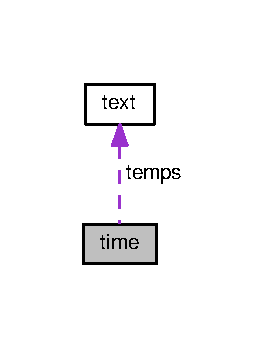
\includegraphics[width=128pt]{structtime__coll__graph}
\end{center}
\end{figure}
\subsection*{Data Fields}
\begin{DoxyCompactItemize}
\item 
int {\bfseries tempsdebut}\hypertarget{structtime_a631b29da38929a12fb4997cb6c77ca65}{}\label{structtime_a631b29da38929a12fb4997cb6c77ca65}

\item 
int {\bfseries mm}\hypertarget{structtime_ae3e68d8be9d3f14dec119d67b848fc47}{}\label{structtime_ae3e68d8be9d3f14dec119d67b848fc47}

\item 
int {\bfseries ss}\hypertarget{structtime_a9d94f0d593508ac616752cbe36601004}{}\label{structtime_a9d94f0d593508ac616752cbe36601004}

\item 
\hyperlink{structtext}{Text} {\bfseries temps}\hypertarget{structtime_a664308034ded61bae3412c574ad3305c}{}\label{structtime_a664308034ded61bae3412c574ad3305c}

\end{DoxyCompactItemize}


The documentation for this struct was generated from the following file\+:\begin{DoxyCompactItemize}
\item 
lot4/type.\+h\end{DoxyCompactItemize}

\chapter{File Documentation}
\hypertarget{background_8c}{}\section{background.\+c File Reference}
\label{background_8c}\index{background.\+c@{background.\+c}}
{\ttfamily \#include \char`\"{}type.\+h\char`\"{}}\\*
Include dependency graph for background.\+c\+:
\nopagebreak
\begin{figure}[H]
\begin{center}
\leavevmode
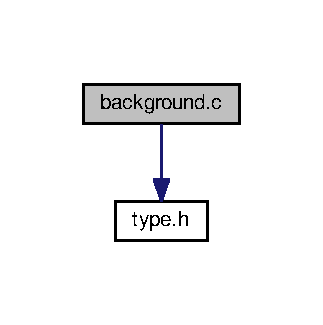
\includegraphics[width=155pt]{background_8c__incl}
\end{center}
\end{figure}
This graph shows which files directly or indirectly include this file\+:
\nopagebreak
\begin{figure}[H]
\begin{center}
\leavevmode
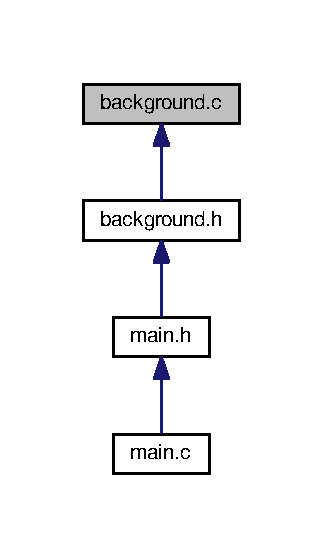
\includegraphics[width=155pt]{background_8c__dep__incl}
\end{center}
\end{figure}
\subsection*{Functions}
\begin{DoxyCompactItemize}
\item 
void {\bfseries Init\+Background} (\hyperlink{structbackground}{background} $\ast$b)\hypertarget{background_8c_a1d2a3dd52321a899b4b7892ce51c4ab0}{}\label{background_8c_a1d2a3dd52321a899b4b7892ce51c4ab0}

\end{DoxyCompactItemize}

\hypertarget{enemy_8c}{}\section{enemy.\+c File Reference}
\label{enemy_8c}\index{enemy.\+c@{enemy.\+c}}
{\ttfamily \#include \char`\"{}type.\+h\char`\"{}}\\*
Include dependency graph for enemy.\+c\+:
\nopagebreak
\begin{figure}[H]
\begin{center}
\leavevmode
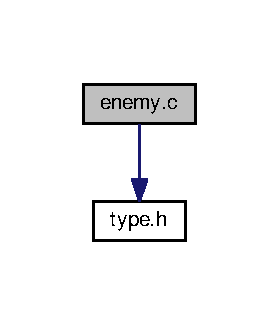
\includegraphics[width=134pt]{enemy_8c__incl}
\end{center}
\end{figure}
This graph shows which files directly or indirectly include this file\+:
\nopagebreak
\begin{figure}[H]
\begin{center}
\leavevmode
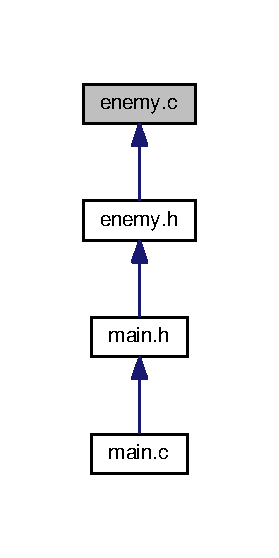
\includegraphics[width=134pt]{enemy_8c__dep__incl}
\end{center}
\end{figure}
\subsection*{Functions}
\begin{DoxyCompactItemize}
\item 
void \hyperlink{enemy_8c_a8ba1f6f3085095b5d01a4c52d30797c7}{init\+Enemy} (\hyperlink{structenemy}{enemy} $\ast$e)
\begin{DoxyCompactList}\small\item\em To initialize Enemy . \end{DoxyCompactList}\item 
void \hyperlink{enemy_8c_a02d7b7a6b7bffad0194e3561b2d938ba}{Deplacement\+Enemy} (\hyperlink{structenemy}{enemy} $\ast$e, \hyperlink{structPersonne}{Personne} p, int $\ast$colone2, int $\ast$ligne2)
\begin{DoxyCompactList}\small\item\em Deplacement AI . \end{DoxyCompactList}\item 
void \hyperlink{enemy_8c_ab9ae1cc50f19979fc2df6ee70d9626b7}{Enemy\+Attack} (\hyperlink{structenemy}{enemy} e, \hyperlink{structPersonne}{Personne} p, int $\ast$colone2, int $\ast$ligne2, int $\ast$S\+T\+OP, int $\ast$Hurt)
\begin{DoxyCompactList}\small\item\em Enemy Attack . \end{DoxyCompactList}\item 
void \hyperlink{enemy_8c_a25b0e4dacc545828c42455fec6260818}{hurtperso} (int $\ast$ligne, int $\ast$colone, int $\ast$hurt)
\begin{DoxyCompactList}\small\item\em Perso Hurt . \end{DoxyCompactList}\item 
void \hyperlink{enemy_8c_a606fc9e18511013d83732b4f8b5b6fce}{Enemy\+Death} (\hyperlink{structenemy}{enemy} e, \hyperlink{structPersonne}{Personne} p, int $\ast$Blit\+Enemy, int ligne)
\begin{DoxyCompactList}\small\item\em Enemy Death . \end{DoxyCompactList}\item 
void \hyperlink{enemy_8c_ab812bb33b0347491dc004a6b06f9fc1f}{deplacement\+\_\+enemy\+\_\+aleatoire} (\hyperlink{structenemy}{enemy} $\ast$e)
\begin{DoxyCompactList}\small\item\em Deplacement Aleatoire . \end{DoxyCompactList}\item 
void {\bfseries Enemy\+Death2} (\hyperlink{structPersonne}{Personne} p1, \hyperlink{structenemy}{enemy} e1, int $\ast$Blit\+Enemy1, int ligne1)\hypertarget{enemy_8c_aae0c2e281bdb77213615af25387a0062}{}\label{enemy_8c_aae0c2e281bdb77213615af25387a0062}

\end{DoxyCompactItemize}


\subsection{Function Documentation}
\index{enemy.\+c@{enemy.\+c}!deplacement\+\_\+enemy\+\_\+aleatoire@{deplacement\+\_\+enemy\+\_\+aleatoire}}
\index{deplacement\+\_\+enemy\+\_\+aleatoire@{deplacement\+\_\+enemy\+\_\+aleatoire}!enemy.\+c@{enemy.\+c}}
\subsubsection[{\texorpdfstring{deplacement\+\_\+enemy\+\_\+aleatoire(enemy $\ast$e)}{deplacement_enemy_aleatoire(enemy *e)}}]{\setlength{\rightskip}{0pt plus 5cm}void deplacement\+\_\+enemy\+\_\+aleatoire (
\begin{DoxyParamCaption}
\item[{{\bf enemy} $\ast$}]{e}
\end{DoxyParamCaption}
)}\hypertarget{enemy_8c_ab812bb33b0347491dc004a6b06f9fc1f}{}\label{enemy_8c_ab812bb33b0347491dc004a6b06f9fc1f}


Deplacement Aleatoire . 

\begin{DoxyReturn}{Returns}
Nothing 
\end{DoxyReturn}


Here is the caller graph for this function\+:
\nopagebreak
\begin{figure}[H]
\begin{center}
\leavevmode
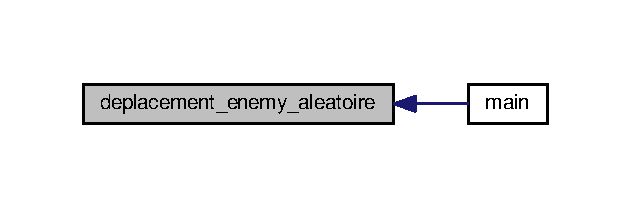
\includegraphics[width=303pt]{enemy_8c_ab812bb33b0347491dc004a6b06f9fc1f_icgraph}
\end{center}
\end{figure}


\index{enemy.\+c@{enemy.\+c}!Deplacement\+Enemy@{Deplacement\+Enemy}}
\index{Deplacement\+Enemy@{Deplacement\+Enemy}!enemy.\+c@{enemy.\+c}}
\subsubsection[{\texorpdfstring{Deplacement\+Enemy(enemy $\ast$e, Personne p, int $\ast$colone2, int $\ast$ligne2)}{DeplacementEnemy(enemy *e, Personne p, int *colone2, int *ligne2)}}]{\setlength{\rightskip}{0pt plus 5cm}void Deplacement\+Enemy (
\begin{DoxyParamCaption}
\item[{{\bf enemy} $\ast$}]{e, }
\item[{{\bf Personne}}]{p, }
\item[{int $\ast$}]{colone2, }
\item[{int $\ast$}]{ligne2}
\end{DoxyParamCaption}
)}\hypertarget{enemy_8c_a02d7b7a6b7bffad0194e3561b2d938ba}{}\label{enemy_8c_a02d7b7a6b7bffad0194e3561b2d938ba}


Deplacement AI . 

\begin{DoxyReturn}{Returns}
Nothing 
\end{DoxyReturn}


Here is the caller graph for this function\+:
\nopagebreak
\begin{figure}[H]
\begin{center}
\leavevmode
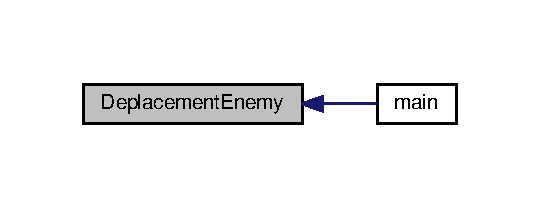
\includegraphics[width=259pt]{enemy_8c_a02d7b7a6b7bffad0194e3561b2d938ba_icgraph}
\end{center}
\end{figure}


\index{enemy.\+c@{enemy.\+c}!Enemy\+Attack@{Enemy\+Attack}}
\index{Enemy\+Attack@{Enemy\+Attack}!enemy.\+c@{enemy.\+c}}
\subsubsection[{\texorpdfstring{Enemy\+Attack(enemy e, Personne p, int $\ast$colone2, int $\ast$ligne2, int $\ast$\+S\+T\+O\+P, int $\ast$\+Hurt)}{EnemyAttack(enemy e, Personne p, int *colone2, int *ligne2, int *STOP, int *Hurt)}}]{\setlength{\rightskip}{0pt plus 5cm}void Enemy\+Attack (
\begin{DoxyParamCaption}
\item[{{\bf enemy}}]{e, }
\item[{{\bf Personne}}]{p, }
\item[{int $\ast$}]{colone2, }
\item[{int $\ast$}]{ligne2, }
\item[{int $\ast$}]{S\+T\+OP, }
\item[{int $\ast$}]{Hurt}
\end{DoxyParamCaption}
)}\hypertarget{enemy_8c_ab9ae1cc50f19979fc2df6ee70d9626b7}{}\label{enemy_8c_ab9ae1cc50f19979fc2df6ee70d9626b7}


Enemy Attack . 

\begin{DoxyReturn}{Returns}
Nothing 
\end{DoxyReturn}


Here is the caller graph for this function\+:
\nopagebreak
\begin{figure}[H]
\begin{center}
\leavevmode
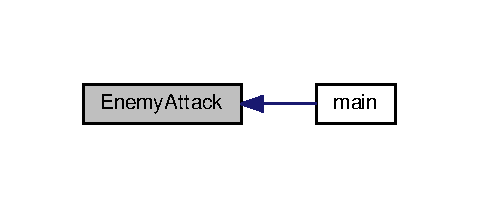
\includegraphics[width=230pt]{enemy_8c_ab9ae1cc50f19979fc2df6ee70d9626b7_icgraph}
\end{center}
\end{figure}


\index{enemy.\+c@{enemy.\+c}!Enemy\+Death@{Enemy\+Death}}
\index{Enemy\+Death@{Enemy\+Death}!enemy.\+c@{enemy.\+c}}
\subsubsection[{\texorpdfstring{Enemy\+Death(enemy e, Personne p, int $\ast$\+Blit\+Enemy, int ligne)}{EnemyDeath(enemy e, Personne p, int *BlitEnemy, int ligne)}}]{\setlength{\rightskip}{0pt plus 5cm}void Enemy\+Death (
\begin{DoxyParamCaption}
\item[{{\bf enemy}}]{e, }
\item[{{\bf Personne}}]{p, }
\item[{int $\ast$}]{Blit\+Enemy, }
\item[{int}]{ligne}
\end{DoxyParamCaption}
)}\hypertarget{enemy_8c_a606fc9e18511013d83732b4f8b5b6fce}{}\label{enemy_8c_a606fc9e18511013d83732b4f8b5b6fce}


Enemy Death . 

\begin{DoxyReturn}{Returns}
Nothing 
\end{DoxyReturn}


Here is the caller graph for this function\+:
\nopagebreak
\begin{figure}[H]
\begin{center}
\leavevmode
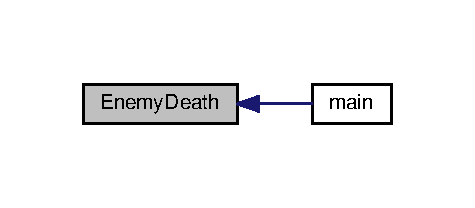
\includegraphics[width=228pt]{enemy_8c_a606fc9e18511013d83732b4f8b5b6fce_icgraph}
\end{center}
\end{figure}


\index{enemy.\+c@{enemy.\+c}!hurtperso@{hurtperso}}
\index{hurtperso@{hurtperso}!enemy.\+c@{enemy.\+c}}
\subsubsection[{\texorpdfstring{hurtperso(int $\ast$ligne, int $\ast$colone, int $\ast$hurt)}{hurtperso(int *ligne, int *colone, int *hurt)}}]{\setlength{\rightskip}{0pt plus 5cm}void hurtperso (
\begin{DoxyParamCaption}
\item[{int $\ast$}]{ligne, }
\item[{int $\ast$}]{colone, }
\item[{int $\ast$}]{hurt}
\end{DoxyParamCaption}
)}\hypertarget{enemy_8c_a25b0e4dacc545828c42455fec6260818}{}\label{enemy_8c_a25b0e4dacc545828c42455fec6260818}


Perso Hurt . 

\begin{DoxyReturn}{Returns}
Nothing 
\end{DoxyReturn}


Here is the caller graph for this function\+:
\nopagebreak
\begin{figure}[H]
\begin{center}
\leavevmode
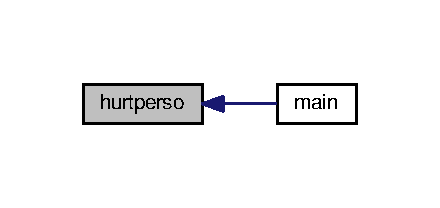
\includegraphics[width=211pt]{enemy_8c_a25b0e4dacc545828c42455fec6260818_icgraph}
\end{center}
\end{figure}


\index{enemy.\+c@{enemy.\+c}!init\+Enemy@{init\+Enemy}}
\index{init\+Enemy@{init\+Enemy}!enemy.\+c@{enemy.\+c}}
\subsubsection[{\texorpdfstring{init\+Enemy(enemy $\ast$e)}{initEnemy(enemy *e)}}]{\setlength{\rightskip}{0pt plus 5cm}void init\+Enemy (
\begin{DoxyParamCaption}
\item[{{\bf enemy} $\ast$}]{e}
\end{DoxyParamCaption}
)}\hypertarget{enemy_8c_a8ba1f6f3085095b5d01a4c52d30797c7}{}\label{enemy_8c_a8ba1f6f3085095b5d01a4c52d30797c7}


To initialize Enemy . 


\begin{DoxyParams}{Parameters}
{\em e} & the enemy \\
\hline
{\em url} & the url of the image \\
\hline
\end{DoxyParams}
\begin{DoxyReturn}{Returns}
Nothing 
\end{DoxyReturn}


Here is the caller graph for this function\+:
\nopagebreak
\begin{figure}[H]
\begin{center}
\leavevmode
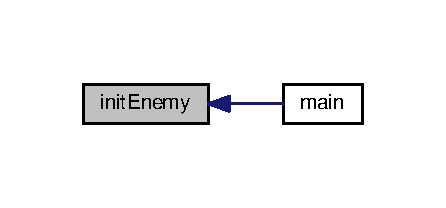
\includegraphics[width=214pt]{enemy_8c_a8ba1f6f3085095b5d01a4c52d30797c7_icgraph}
\end{center}
\end{figure}



\hypertarget{enigme_8c}{}\section{enigme.\+c File Reference}
\label{enigme_8c}\index{enigme.\+c@{enigme.\+c}}
{\ttfamily \#include \char`\"{}type.\+h\char`\"{}}\\*
Include dependency graph for enigme.\+c\+:
\nopagebreak
\begin{figure}[H]
\begin{center}
\leavevmode
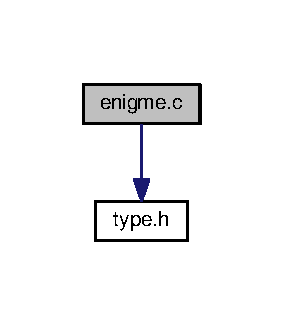
\includegraphics[width=136pt]{enigme_8c__incl}
\end{center}
\end{figure}
This graph shows which files directly or indirectly include this file\+:
\nopagebreak
\begin{figure}[H]
\begin{center}
\leavevmode
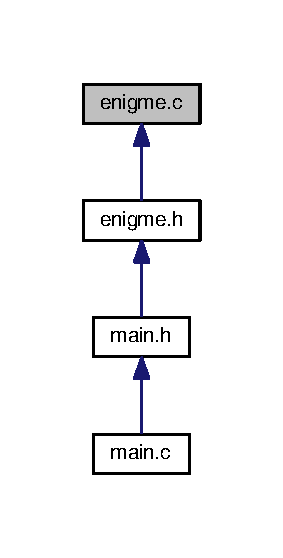
\includegraphics[width=136pt]{enigme_8c__dep__incl}
\end{center}
\end{figure}
\subsection*{Functions}
\begin{DoxyCompactItemize}
\item 
void {\bfseries solution} (S\+D\+L\+\_\+\+Surface $\ast$ecran, int d)\hypertarget{enigme_8c_a2774260562b0dca66057190a74a45edb}{}\label{enigme_8c_a2774260562b0dca66057190a74a45edb}

\item 
void \hyperlink{enigme_8c_a859263f14512437b6ccdfb54535a6875}{correct} (S\+D\+L\+\_\+\+Surface $\ast$ecran)
\begin{DoxyCompactList}\small\item\em Correct Answers . \end{DoxyCompactList}\item 
void \hyperlink{enigme_8c_ad0c551a5e3c3dd1cf60f35fef5a31e32}{enigma} (S\+D\+L\+\_\+\+Surface $\ast$ecran, int d)
\begin{DoxyCompactList}\small\item\em Blit Enigme . \end{DoxyCompactList}\item 
int \hyperlink{enigme_8c_a72498611e7543eea612c9ff46eb1ce01}{reponse} (S\+D\+L\+\_\+\+Surface $\ast$ecran, int d)
\begin{DoxyCompactList}\small\item\em Answers . \end{DoxyCompactList}\item 
int \hyperlink{enigme_8c_adf5359e458145728c485621cdc63b620}{Enigme} ()
\begin{DoxyCompactList}\small\item\em To initialize Enigme . \end{DoxyCompactList}\end{DoxyCompactItemize}


\subsection{Function Documentation}
\index{enigme.\+c@{enigme.\+c}!correct@{correct}}
\index{correct@{correct}!enigme.\+c@{enigme.\+c}}
\subsubsection[{\texorpdfstring{correct(\+S\+D\+L\+\_\+\+Surface $\ast$ecran)}{correct(SDL_Surface *ecran)}}]{\setlength{\rightskip}{0pt plus 5cm}void correct (
\begin{DoxyParamCaption}
\item[{S\+D\+L\+\_\+\+Surface $\ast$}]{ecran}
\end{DoxyParamCaption}
)}\hypertarget{enigme_8c_a859263f14512437b6ccdfb54535a6875}{}\label{enigme_8c_a859263f14512437b6ccdfb54535a6875}


Correct Answers . 

\begin{DoxyReturn}{Returns}
Nothing 
\end{DoxyReturn}


Here is the caller graph for this function\+:
\nopagebreak
\begin{figure}[H]
\begin{center}
\leavevmode
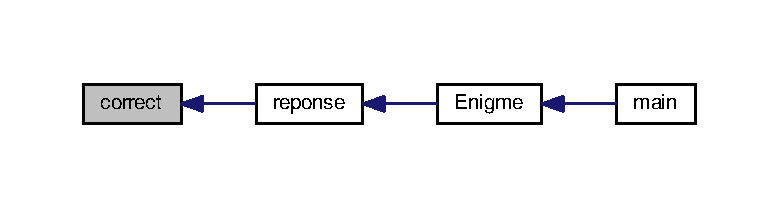
\includegraphics[width=350pt]{enigme_8c_a859263f14512437b6ccdfb54535a6875_icgraph}
\end{center}
\end{figure}


\index{enigme.\+c@{enigme.\+c}!enigma@{enigma}}
\index{enigma@{enigma}!enigme.\+c@{enigme.\+c}}
\subsubsection[{\texorpdfstring{enigma(\+S\+D\+L\+\_\+\+Surface $\ast$ecran, int d)}{enigma(SDL_Surface *ecran, int d)}}]{\setlength{\rightskip}{0pt plus 5cm}void enigma (
\begin{DoxyParamCaption}
\item[{S\+D\+L\+\_\+\+Surface $\ast$}]{ecran, }
\item[{int}]{d}
\end{DoxyParamCaption}
)}\hypertarget{enigme_8c_ad0c551a5e3c3dd1cf60f35fef5a31e32}{}\label{enigme_8c_ad0c551a5e3c3dd1cf60f35fef5a31e32}


Blit Enigme . 

\begin{DoxyReturn}{Returns}
Nothing 
\end{DoxyReturn}


Here is the caller graph for this function\+:
\nopagebreak
\begin{figure}[H]
\begin{center}
\leavevmode
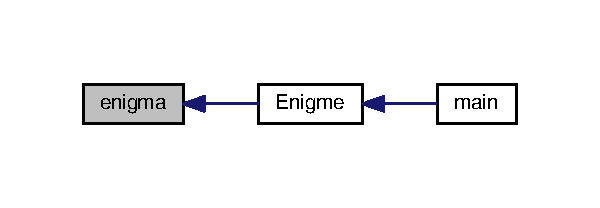
\includegraphics[width=288pt]{enigme_8c_ad0c551a5e3c3dd1cf60f35fef5a31e32_icgraph}
\end{center}
\end{figure}


\index{enigme.\+c@{enigme.\+c}!Enigme@{Enigme}}
\index{Enigme@{Enigme}!enigme.\+c@{enigme.\+c}}
\subsubsection[{\texorpdfstring{Enigme()}{Enigme()}}]{\setlength{\rightskip}{0pt plus 5cm}int Enigme (
\begin{DoxyParamCaption}
{}
\end{DoxyParamCaption}
)}\hypertarget{enigme_8c_adf5359e458145728c485621cdc63b620}{}\label{enigme_8c_adf5359e458145728c485621cdc63b620}


To initialize Enigme . 

\begin{DoxyReturn}{Returns}
Nothing 
\end{DoxyReturn}


Here is the call graph for this function\+:
\nopagebreak
\begin{figure}[H]
\begin{center}
\leavevmode
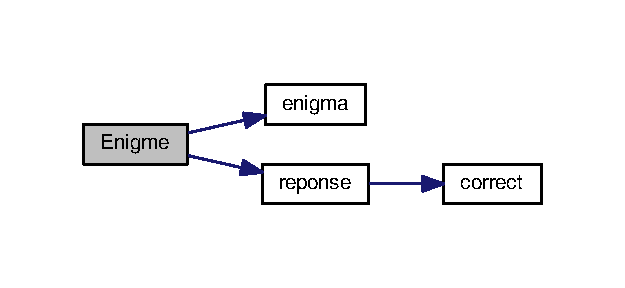
\includegraphics[width=300pt]{enigme_8c_adf5359e458145728c485621cdc63b620_cgraph}
\end{center}
\end{figure}




Here is the caller graph for this function\+:
\nopagebreak
\begin{figure}[H]
\begin{center}
\leavevmode
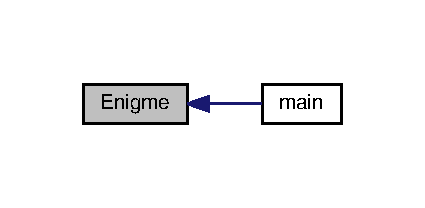
\includegraphics[width=204pt]{enigme_8c_adf5359e458145728c485621cdc63b620_icgraph}
\end{center}
\end{figure}


\index{enigme.\+c@{enigme.\+c}!reponse@{reponse}}
\index{reponse@{reponse}!enigme.\+c@{enigme.\+c}}
\subsubsection[{\texorpdfstring{reponse(\+S\+D\+L\+\_\+\+Surface $\ast$ecran, int d)}{reponse(SDL_Surface *ecran, int d)}}]{\setlength{\rightskip}{0pt plus 5cm}int reponse (
\begin{DoxyParamCaption}
\item[{S\+D\+L\+\_\+\+Surface $\ast$}]{ecran, }
\item[{int}]{d}
\end{DoxyParamCaption}
)}\hypertarget{enigme_8c_a72498611e7543eea612c9ff46eb1ce01}{}\label{enigme_8c_a72498611e7543eea612c9ff46eb1ce01}


Answers . 

\begin{DoxyReturn}{Returns}
Nothing 
\end{DoxyReturn}


Here is the call graph for this function\+:
\nopagebreak
\begin{figure}[H]
\begin{center}
\leavevmode
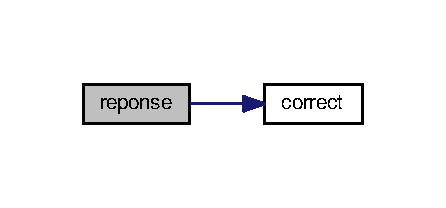
\includegraphics[width=214pt]{enigme_8c_a72498611e7543eea612c9ff46eb1ce01_cgraph}
\end{center}
\end{figure}




Here is the caller graph for this function\+:
\nopagebreak
\begin{figure}[H]
\begin{center}
\leavevmode
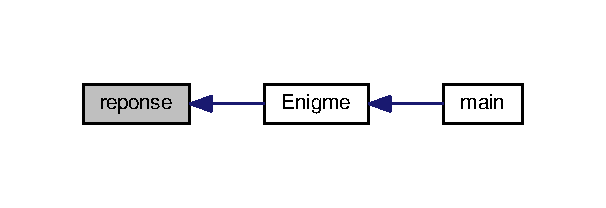
\includegraphics[width=291pt]{enigme_8c_a72498611e7543eea612c9ff46eb1ce01_icgraph}
\end{center}
\end{figure}



\hypertarget{enigmealeatoire_8c}{}\section{enigmealeatoire.\+c File Reference}
\label{enigmealeatoire_8c}\index{enigmealeatoire.\+c@{enigmealeatoire.\+c}}
{\ttfamily \#include \char`\"{}type.\+h\char`\"{}}\\*
Include dependency graph for enigmealeatoire.\+c\+:
\nopagebreak
\begin{figure}[H]
\begin{center}
\leavevmode
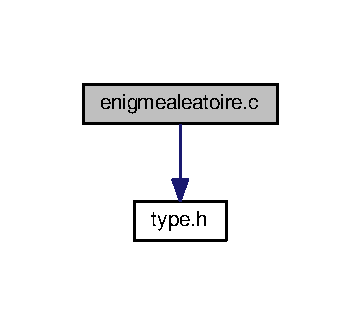
\includegraphics[width=173pt]{enigmealeatoire_8c__incl}
\end{center}
\end{figure}
This graph shows which files directly or indirectly include this file\+:
\nopagebreak
\begin{figure}[H]
\begin{center}
\leavevmode
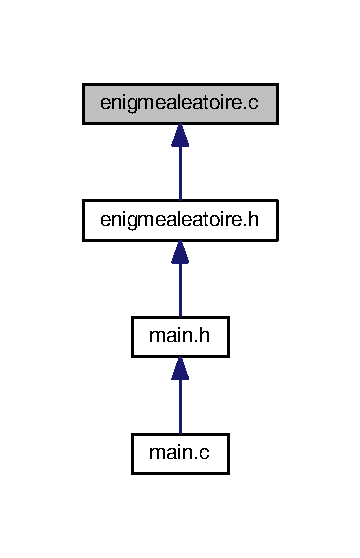
\includegraphics[width=173pt]{enigmealeatoire_8c__dep__incl}
\end{center}
\end{figure}
\subsection*{Functions}
\begin{DoxyCompactItemize}
\item 
void {\bfseries init\+\_\+enigme} (\hyperlink{structenigme}{enigme} $\ast$e)\hypertarget{enigmealeatoire_8c_a194546ea4fa1a0eaa63aacbac96f33bb}{}\label{enigmealeatoire_8c_a194546ea4fa1a0eaa63aacbac96f33bb}

\item 
\hyperlink{structenigme}{enigme} {\bfseries generer} ()\hypertarget{enigmealeatoire_8c_a36dc0cbc075842d7ed4c5c209031a978}{}\label{enigmealeatoire_8c_a36dc0cbc075842d7ed4c5c209031a978}

\item 
void {\bfseries afficherenigme} (\hyperlink{structenigme}{enigme} e, S\+D\+L\+\_\+\+Surface $\ast$ecran)\hypertarget{enigmealeatoire_8c_ac16d8f79b694c6921c49974fae27c90d}{}\label{enigmealeatoire_8c_ac16d8f79b694c6921c49974fae27c90d}

\item 
void {\bfseries affichage\+\_\+repvraie} (S\+D\+L\+\_\+\+Surface $\ast$ecran, \hyperlink{structenigme}{enigme} e)\hypertarget{enigmealeatoire_8c_aaee92bd6a9f7ff8b6312c0041a549d98}{}\label{enigmealeatoire_8c_aaee92bd6a9f7ff8b6312c0041a549d98}

\item 
void {\bfseries affichage\+\_\+repfausse} (S\+D\+L\+\_\+\+Surface $\ast$ecran, \hyperlink{structenigme}{enigme} e)\hypertarget{enigmealeatoire_8c_a554cc9e01566b8c241ef6708a29d3fa5}{}\label{enigmealeatoire_8c_a554cc9e01566b8c241ef6708a29d3fa5}

\item 
int {\bfseries Enigme\+Sans\+Fichier} ()\hypertarget{enigmealeatoire_8c_a226e6d4490a6d78793bfa5d9455b5f5f}{}\label{enigmealeatoire_8c_a226e6d4490a6d78793bfa5d9455b5f5f}

\end{DoxyCompactItemize}

\hypertarget{main_8c}{}\section{main.\+c File Reference}
\label{main_8c}\index{main.\+c@{main.\+c}}


Testing Program.  


{\ttfamily \#include \char`\"{}main.\+h\char`\"{}}\\*
Include dependency graph for main.\+c\+:
\nopagebreak
\begin{figure}[H]
\begin{center}
\leavevmode
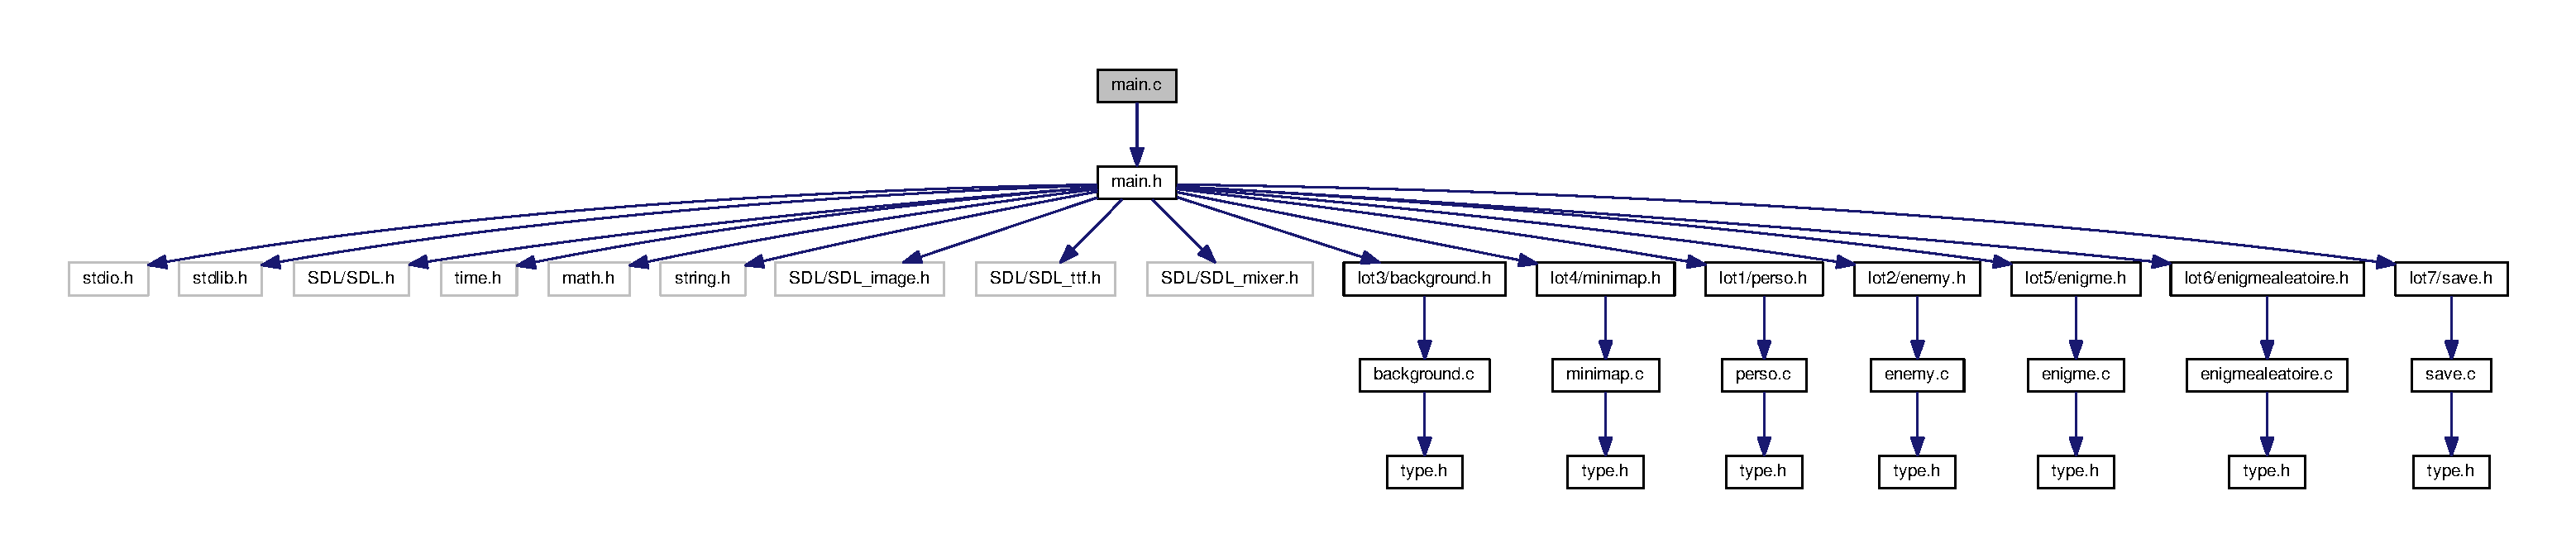
\includegraphics[width=350pt]{main_8c__incl}
\end{center}
\end{figure}
\subsection*{Functions}
\begin{DoxyCompactItemize}
\item 
void \hyperlink{main_8c_acdef7a1fd863a6d3770c1268cb06add3}{main} ()
\end{DoxyCompactItemize}


\subsection{Detailed Description}
Testing Program. 

\begin{DoxyAuthor}{Author}
W\+Alid jlassi 
\end{DoxyAuthor}
\begin{DoxyVersion}{Version}
0.\+1 
\end{DoxyVersion}
\begin{DoxyDate}{Date}
Apr 21, 2021
\end{DoxyDate}
Testing program for background scrollilng $\ast$ 

\subsection{Function Documentation}
\index{main.\+c@{main.\+c}!main@{main}}
\index{main@{main}!main.\+c@{main.\+c}}
\subsubsection[{\texorpdfstring{main()}{main()}}]{\setlength{\rightskip}{0pt plus 5cm}void main (
\begin{DoxyParamCaption}
{}
\end{DoxyParamCaption}
)}\hypertarget{main_8c_acdef7a1fd863a6d3770c1268cb06add3}{}\label{main_8c_acdef7a1fd863a6d3770c1268cb06add3}
8///////////////////////////////// B\+A\+C\+K\+G\+R\+O\+U\+N\+D///

minimap

milieu de ecran///

enemy///

time///

M\+E\+N\+U/// 

Here is the call graph for this function\+:
\nopagebreak
\begin{figure}[H]
\begin{center}
\leavevmode
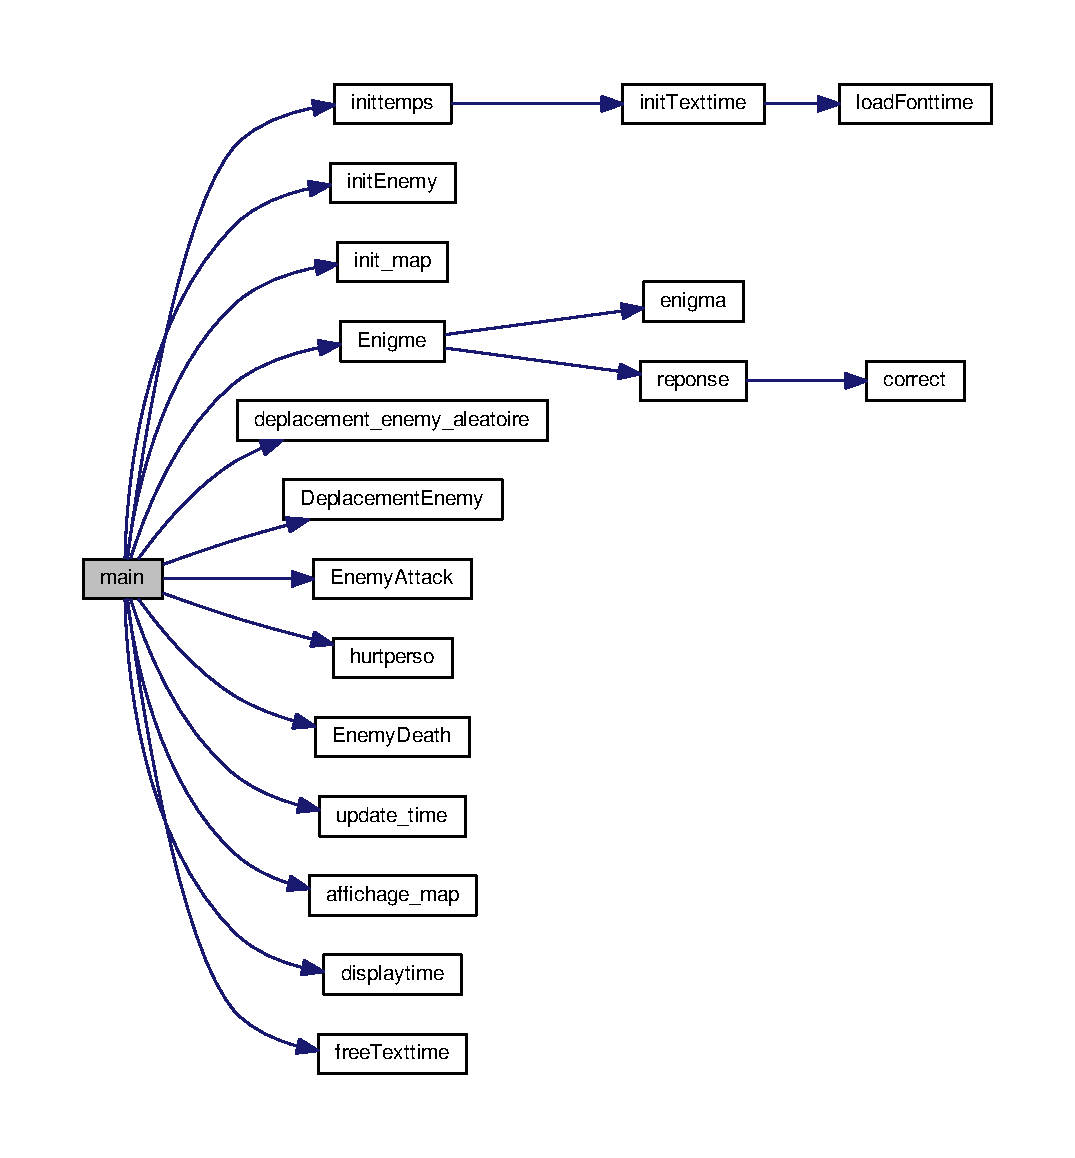
\includegraphics[width=350pt]{main_8c_acdef7a1fd863a6d3770c1268cb06add3_cgraph}
\end{center}
\end{figure}



\hypertarget{minimap_8c}{}\section{minimap.\+c File Reference}
\label{minimap_8c}\index{minimap.\+c@{minimap.\+c}}
{\ttfamily \#include \char`\"{}type.\+h\char`\"{}}\\*
Include dependency graph for minimap.\+c\+:
\nopagebreak
\begin{figure}[H]
\begin{center}
\leavevmode
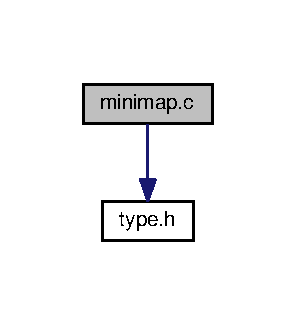
\includegraphics[width=142pt]{minimap_8c__incl}
\end{center}
\end{figure}
This graph shows which files directly or indirectly include this file\+:
\nopagebreak
\begin{figure}[H]
\begin{center}
\leavevmode
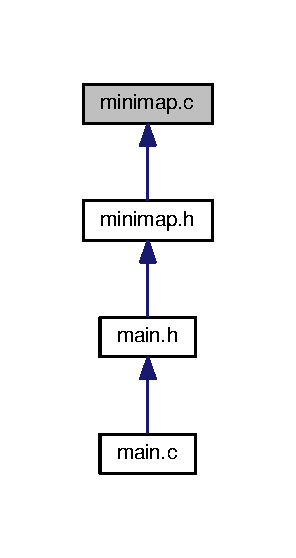
\includegraphics[width=142pt]{minimap_8c__dep__incl}
\end{center}
\end{figure}
\subsection*{Functions}
\begin{DoxyCompactItemize}
\item 
void \hyperlink{minimap_8c_a74ec4a47290d0f4cb6091de5aa33e0fa}{init\+\_\+map} (\hyperlink{structminimap}{minimap} $\ast$m)
\begin{DoxyCompactList}\small\item\em To initialize The minimap . \end{DoxyCompactList}\item 
void \hyperlink{minimap_8c_a71c8c908c2ec624cd28536ebf0919f19}{affichage\+\_\+map} (\hyperlink{structminimap}{minimap} m, S\+D\+L\+\_\+\+Surface $\ast$screen)
\begin{DoxyCompactList}\small\item\em Blit the Minimap . \end{DoxyCompactList}\item 
void {\bfseries Timer} (int $\ast$tempsdebut)\hypertarget{minimap_8c_a5929c26a66049460dc58b8c92a6d0b2f}{}\label{minimap_8c_a5929c26a66049460dc58b8c92a6d0b2f}

\item 
int \hyperlink{minimap_8c_adbaf68f859776c327cf59e5f78f25627}{load\+Fonttime} (\hyperlink{structtext}{Text} $\ast$T, char $\ast$ch)
\begin{DoxyCompactList}\small\item\em load\+Fonttime \end{DoxyCompactList}\item 
int \hyperlink{minimap_8c_ae326325c6cbb8e991873fc3da6a8265e}{init\+Texttime} (\hyperlink{structtext}{Text} $\ast$T)
\begin{DoxyCompactList}\small\item\em To initialize the time . \end{DoxyCompactList}\item 
void \hyperlink{minimap_8c_a2bbd14a997f1fa7fd246f24ead3b50f8}{inittemps} (\hyperlink{structtime}{Time} $\ast$t)
\begin{DoxyCompactList}\small\item\em To initialize the texttime. \end{DoxyCompactList}\item 
void \hyperlink{minimap_8c_abc558b87e2e48a9f354536407ee6abbd}{update\+\_\+time} (\hyperlink{structtime}{Time} $\ast$T)
\begin{DoxyCompactList}\small\item\em update\+\_\+time \end{DoxyCompactList}\item 
void \hyperlink{minimap_8c_aeaf577c70c6195dd63b6424c46025020}{displaytime} (\hyperlink{structtime}{Time} T, S\+D\+L\+\_\+\+Surface $\ast$screen)
\begin{DoxyCompactList}\small\item\em displaytime \end{DoxyCompactList}\item 
void \hyperlink{minimap_8c_a1aea230c66513887e2a8dba8b3d2d075}{free\+Texttime} (\hyperlink{structtext}{Text} T)
\begin{DoxyCompactList}\small\item\em free\+Texttime \end{DoxyCompactList}\end{DoxyCompactItemize}


\subsection{Function Documentation}
\index{minimap.\+c@{minimap.\+c}!affichage\+\_\+map@{affichage\+\_\+map}}
\index{affichage\+\_\+map@{affichage\+\_\+map}!minimap.\+c@{minimap.\+c}}
\subsubsection[{\texorpdfstring{affichage\+\_\+map(minimap m, S\+D\+L\+\_\+\+Surface $\ast$screen)}{affichage_map(minimap m, SDL_Surface *screen)}}]{\setlength{\rightskip}{0pt plus 5cm}void affichage\+\_\+map (
\begin{DoxyParamCaption}
\item[{{\bf minimap}}]{m, }
\item[{S\+D\+L\+\_\+\+Surface $\ast$}]{screen}
\end{DoxyParamCaption}
)}\hypertarget{minimap_8c_a71c8c908c2ec624cd28536ebf0919f19}{}\label{minimap_8c_a71c8c908c2ec624cd28536ebf0919f19}


Blit the Minimap . 

\begin{DoxyReturn}{Returns}
Nothing 
\end{DoxyReturn}


Here is the caller graph for this function\+:
\nopagebreak
\begin{figure}[H]
\begin{center}
\leavevmode
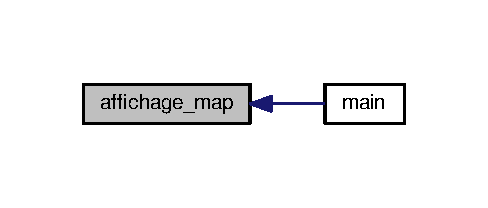
\includegraphics[width=234pt]{minimap_8c_a71c8c908c2ec624cd28536ebf0919f19_icgraph}
\end{center}
\end{figure}


\index{minimap.\+c@{minimap.\+c}!displaytime@{displaytime}}
\index{displaytime@{displaytime}!minimap.\+c@{minimap.\+c}}
\subsubsection[{\texorpdfstring{displaytime(\+Time T, S\+D\+L\+\_\+\+Surface $\ast$screen)}{displaytime(Time T, SDL_Surface *screen)}}]{\setlength{\rightskip}{0pt plus 5cm}void displaytime (
\begin{DoxyParamCaption}
\item[{{\bf Time}}]{T, }
\item[{S\+D\+L\+\_\+\+Surface $\ast$}]{screen}
\end{DoxyParamCaption}
)}\hypertarget{minimap_8c_aeaf577c70c6195dd63b6424c46025020}{}\label{minimap_8c_aeaf577c70c6195dd63b6424c46025020}


displaytime 


\begin{DoxyParams}{Parameters}
{\em T} & the Time \\
\hline
{\em screen} & the url surface \\
\hline
\end{DoxyParams}
\begin{DoxyReturn}{Returns}
Nothing 
\end{DoxyReturn}


Here is the caller graph for this function\+:
\nopagebreak
\begin{figure}[H]
\begin{center}
\leavevmode
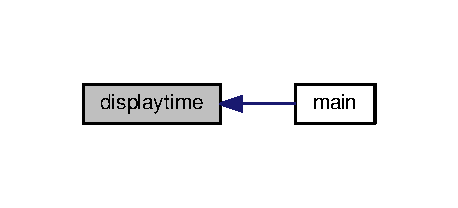
\includegraphics[width=220pt]{minimap_8c_aeaf577c70c6195dd63b6424c46025020_icgraph}
\end{center}
\end{figure}


\index{minimap.\+c@{minimap.\+c}!free\+Texttime@{free\+Texttime}}
\index{free\+Texttime@{free\+Texttime}!minimap.\+c@{minimap.\+c}}
\subsubsection[{\texorpdfstring{free\+Texttime(\+Text T)}{freeTexttime(Text T)}}]{\setlength{\rightskip}{0pt plus 5cm}void free\+Texttime (
\begin{DoxyParamCaption}
\item[{{\bf Text}}]{T}
\end{DoxyParamCaption}
)}\hypertarget{minimap_8c_a1aea230c66513887e2a8dba8b3d2d075}{}\label{minimap_8c_a1aea230c66513887e2a8dba8b3d2d075}


free\+Texttime 


\begin{DoxyParams}{Parameters}
{\em T} & the text \\
\hline
\end{DoxyParams}
\begin{DoxyReturn}{Returns}
Nothing 
\end{DoxyReturn}


Here is the caller graph for this function\+:
\nopagebreak
\begin{figure}[H]
\begin{center}
\leavevmode
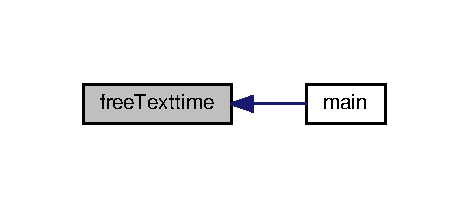
\includegraphics[width=225pt]{minimap_8c_a1aea230c66513887e2a8dba8b3d2d075_icgraph}
\end{center}
\end{figure}


\index{minimap.\+c@{minimap.\+c}!init\+\_\+map@{init\+\_\+map}}
\index{init\+\_\+map@{init\+\_\+map}!minimap.\+c@{minimap.\+c}}
\subsubsection[{\texorpdfstring{init\+\_\+map(minimap $\ast$m)}{init_map(minimap *m)}}]{\setlength{\rightskip}{0pt plus 5cm}void init\+\_\+map (
\begin{DoxyParamCaption}
\item[{{\bf minimap} $\ast$}]{m}
\end{DoxyParamCaption}
)}\hypertarget{minimap_8c_a74ec4a47290d0f4cb6091de5aa33e0fa}{}\label{minimap_8c_a74ec4a47290d0f4cb6091de5aa33e0fa}


To initialize The minimap . 


\begin{DoxyParams}{Parameters}
{\em m} & the minimap \\
\hline
{\em url} & the url of the image \\
\hline
\end{DoxyParams}
\begin{DoxyReturn}{Returns}
Nothing 
\end{DoxyReturn}


Here is the caller graph for this function\+:
\nopagebreak
\begin{figure}[H]
\begin{center}
\leavevmode
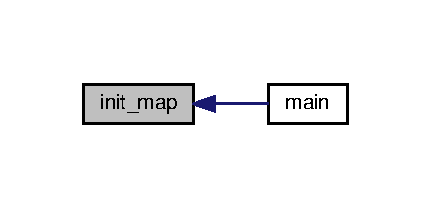
\includegraphics[width=207pt]{minimap_8c_a74ec4a47290d0f4cb6091de5aa33e0fa_icgraph}
\end{center}
\end{figure}


\index{minimap.\+c@{minimap.\+c}!inittemps@{inittemps}}
\index{inittemps@{inittemps}!minimap.\+c@{minimap.\+c}}
\subsubsection[{\texorpdfstring{inittemps(\+Time $\ast$t)}{inittemps(Time *t)}}]{\setlength{\rightskip}{0pt plus 5cm}void inittemps (
\begin{DoxyParamCaption}
\item[{{\bf Time} $\ast$}]{t}
\end{DoxyParamCaption}
)}\hypertarget{minimap_8c_a2bbd14a997f1fa7fd246f24ead3b50f8}{}\label{minimap_8c_a2bbd14a997f1fa7fd246f24ead3b50f8}


To initialize the texttime. 


\begin{DoxyParams}{Parameters}
{\em T} & the text \\
\hline
\end{DoxyParams}
\begin{DoxyReturn}{Returns}
integer 
\end{DoxyReturn}


Here is the call graph for this function\+:
\nopagebreak
\begin{figure}[H]
\begin{center}
\leavevmode
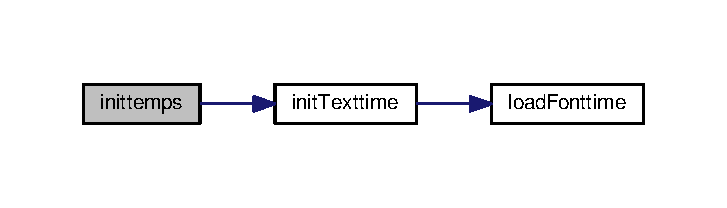
\includegraphics[width=349pt]{minimap_8c_a2bbd14a997f1fa7fd246f24ead3b50f8_cgraph}
\end{center}
\end{figure}




Here is the caller graph for this function\+:
\nopagebreak
\begin{figure}[H]
\begin{center}
\leavevmode
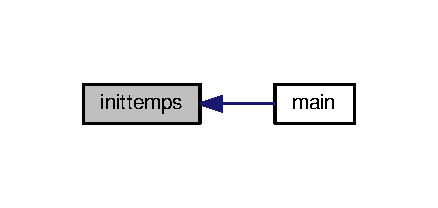
\includegraphics[width=210pt]{minimap_8c_a2bbd14a997f1fa7fd246f24ead3b50f8_icgraph}
\end{center}
\end{figure}


\index{minimap.\+c@{minimap.\+c}!init\+Texttime@{init\+Texttime}}
\index{init\+Texttime@{init\+Texttime}!minimap.\+c@{minimap.\+c}}
\subsubsection[{\texorpdfstring{init\+Texttime(\+Text $\ast$\+T)}{initTexttime(Text *T)}}]{\setlength{\rightskip}{0pt plus 5cm}int init\+Texttime (
\begin{DoxyParamCaption}
\item[{{\bf Text} $\ast$}]{T}
\end{DoxyParamCaption}
)}\hypertarget{minimap_8c_ae326325c6cbb8e991873fc3da6a8265e}{}\label{minimap_8c_ae326325c6cbb8e991873fc3da6a8265e}


To initialize the time . 


\begin{DoxyParams}{Parameters}
{\em t} & the Time \\
\hline
\end{DoxyParams}
\begin{DoxyReturn}{Returns}
Nothing 
\end{DoxyReturn}


Here is the call graph for this function\+:
\nopagebreak
\begin{figure}[H]
\begin{center}
\leavevmode
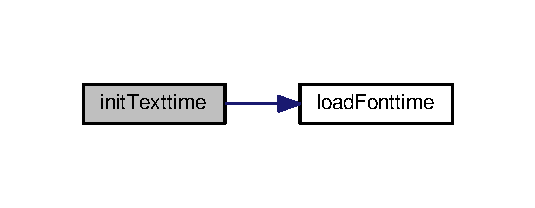
\includegraphics[width=257pt]{minimap_8c_ae326325c6cbb8e991873fc3da6a8265e_cgraph}
\end{center}
\end{figure}




Here is the caller graph for this function\+:
\nopagebreak
\begin{figure}[H]
\begin{center}
\leavevmode
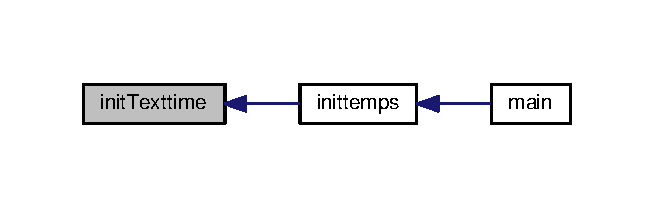
\includegraphics[width=314pt]{minimap_8c_ae326325c6cbb8e991873fc3da6a8265e_icgraph}
\end{center}
\end{figure}


\index{minimap.\+c@{minimap.\+c}!load\+Fonttime@{load\+Fonttime}}
\index{load\+Fonttime@{load\+Fonttime}!minimap.\+c@{minimap.\+c}}
\subsubsection[{\texorpdfstring{load\+Fonttime(\+Text $\ast$\+T, char $\ast$ch)}{loadFonttime(Text *T, char *ch)}}]{\setlength{\rightskip}{0pt plus 5cm}int load\+Fonttime (
\begin{DoxyParamCaption}
\item[{{\bf Text} $\ast$}]{T, }
\item[{char $\ast$}]{ch}
\end{DoxyParamCaption}
)}\hypertarget{minimap_8c_adbaf68f859776c327cf59e5f78f25627}{}\label{minimap_8c_adbaf68f859776c327cf59e5f78f25627}


load\+Fonttime 


\begin{DoxyParams}{Parameters}
{\em T} & the text \\
\hline
{\em ch} & \\
\hline
\end{DoxyParams}
\begin{DoxyReturn}{Returns}
integer 
\end{DoxyReturn}


Here is the caller graph for this function\+:
\nopagebreak
\begin{figure}[H]
\begin{center}
\leavevmode
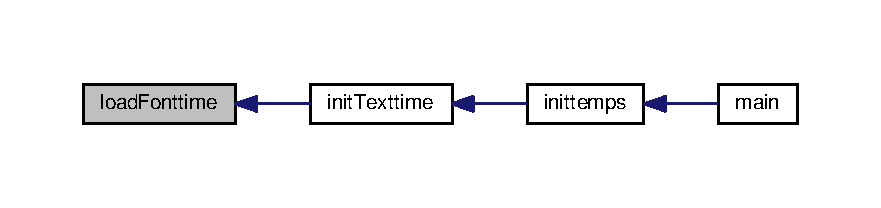
\includegraphics[width=350pt]{minimap_8c_adbaf68f859776c327cf59e5f78f25627_icgraph}
\end{center}
\end{figure}


\index{minimap.\+c@{minimap.\+c}!update\+\_\+time@{update\+\_\+time}}
\index{update\+\_\+time@{update\+\_\+time}!minimap.\+c@{minimap.\+c}}
\subsubsection[{\texorpdfstring{update\+\_\+time(\+Time $\ast$\+T)}{update_time(Time *T)}}]{\setlength{\rightskip}{0pt plus 5cm}void update\+\_\+time (
\begin{DoxyParamCaption}
\item[{{\bf Time} $\ast$}]{T}
\end{DoxyParamCaption}
)}\hypertarget{minimap_8c_abc558b87e2e48a9f354536407ee6abbd}{}\label{minimap_8c_abc558b87e2e48a9f354536407ee6abbd}


update\+\_\+time 


\begin{DoxyParams}{Parameters}
{\em T} & the Time \\
\hline
\end{DoxyParams}
\begin{DoxyReturn}{Returns}
Nothing 
\end{DoxyReturn}


Here is the caller graph for this function\+:
\nopagebreak
\begin{figure}[H]
\begin{center}
\leavevmode
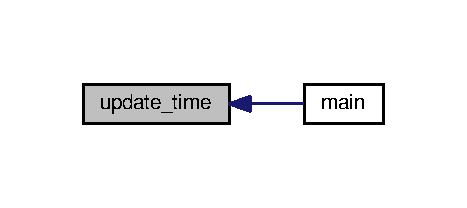
\includegraphics[width=224pt]{minimap_8c_abc558b87e2e48a9f354536407ee6abbd_icgraph}
\end{center}
\end{figure}



\hypertarget{perso_8c}{}\section{perso.\+c File Reference}
\label{perso_8c}\index{perso.\+c@{perso.\+c}}
{\ttfamily \#include \char`\"{}type.\+h\char`\"{}}\\*
Include dependency graph for perso.\+c\+:
\nopagebreak
\begin{figure}[H]
\begin{center}
\leavevmode
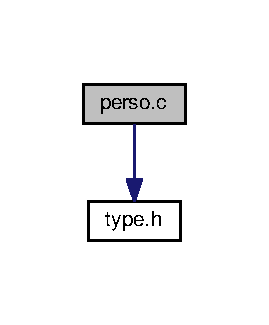
\includegraphics[width=129pt]{perso_8c__incl}
\end{center}
\end{figure}
This graph shows which files directly or indirectly include this file\+:
\nopagebreak
\begin{figure}[H]
\begin{center}
\leavevmode
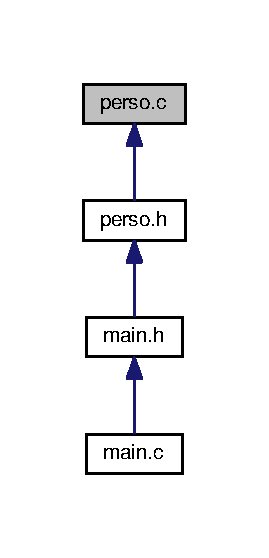
\includegraphics[width=129pt]{perso_8c__dep__incl}
\end{center}
\end{figure}
\subsection*{Functions}
\begin{DoxyCompactItemize}
\item 
void {\bfseries init\+Perso} (\hyperlink{structPersonne}{Personne} $\ast$p)\hypertarget{perso_8c_abda5588ee769d930707712edb58003cd}{}\label{perso_8c_abda5588ee769d930707712edb58003cd}

\item 
void {\bfseries init\+Perso2} (\hyperlink{structPersonne}{Personne} $\ast$p1)\hypertarget{perso_8c_a9d5fde20b720340a60470ef860540a71}{}\label{perso_8c_a9d5fde20b720340a60470ef860540a71}

\item 
void {\bfseries move\+Left} (int $\ast$ligne, \hyperlink{structPersonne}{Personne} $\ast$p, S\+D\+L\+\_\+\+Rect $\ast$Camera, \hyperlink{structminimap}{minimap} $\ast$m)\hypertarget{perso_8c_a69a66be7a6efa2d89f87bf4b569f4fed}{}\label{perso_8c_a69a66be7a6efa2d89f87bf4b569f4fed}

\item 
void {\bfseries move\+Right} (int $\ast$ligne, \hyperlink{structPersonne}{Personne} $\ast$p, S\+D\+L\+\_\+\+Rect $\ast$Camera, \hyperlink{structminimap}{minimap} $\ast$m)\hypertarget{perso_8c_a2696f4f041cfbc0aabacfd428eb075cc}{}\label{perso_8c_a2696f4f041cfbc0aabacfd428eb075cc}

\item 
void {\bfseries sprint} (int $\ast$ligne, \hyperlink{structPersonne}{Personne} $\ast$p, S\+D\+L\+\_\+\+Rect $\ast$Camera)\hypertarget{perso_8c_a19c94d5b70c61962666abdbd6fbcf6f6}{}\label{perso_8c_a19c94d5b70c61962666abdbd6fbcf6f6}

\item 
void {\bfseries stop} (int $\ast$ligne, \hyperlink{structPersonne}{Personne} $\ast$p, S\+D\+L\+\_\+\+Rect $\ast$Camera, int $\ast$acc, int $\ast$colone, int $\ast$done)\hypertarget{perso_8c_ab59dd4f3bc2e70d1eca6e0c4a057e8e3}{}\label{perso_8c_ab59dd4f3bc2e70d1eca6e0c4a057e8e3}

\item 
void {\bfseries jump} (int $\ast$ligne, \hyperlink{structPersonne}{Personne} $\ast$p, S\+D\+L\+\_\+\+Rect $\ast$Camera, int $\ast$acc, \hyperlink{structPersonne}{Personne} $\ast$p1)\hypertarget{perso_8c_a20bd0a77ed9f547959c9cdc0af09452e}{}\label{perso_8c_a20bd0a77ed9f547959c9cdc0af09452e}

\item 
void {\bfseries slap} (int $\ast$ligne, int $\ast$colone, int $\ast$b)\hypertarget{perso_8c_ac1daf537e884edaa579b02e0cc685050}{}\label{perso_8c_ac1daf537e884edaa579b02e0cc685050}

\item 
void {\bfseries ulti} (int $\ast$ligne, int $\ast$colone, int $\ast$ult, \hyperlink{structPersonne}{Personne} $\ast$p)\hypertarget{perso_8c_acfff0420768d145105977bd0a5402042}{}\label{perso_8c_acfff0420768d145105977bd0a5402042}

\item 
void {\bfseries death} (int $\ast$ligne, int $\ast$colone, int $\ast$b, \hyperlink{structPersonne}{Personne} $\ast$p)\hypertarget{perso_8c_a27f41bc7009e82a0bea0d40325df2efd}{}\label{perso_8c_a27f41bc7009e82a0bea0d40325df2efd}

\item 
void {\bfseries afficher\+Perso} (\hyperlink{structPersonne}{Personne} p, int ligne, int colone, S\+D\+L\+\_\+\+Surface $\ast$screen)\hypertarget{perso_8c_afb2826f7564d401adb7ba648cb3f94d7}{}\label{perso_8c_afb2826f7564d401adb7ba648cb3f94d7}

\end{DoxyCompactItemize}

\hypertarget{save_8c}{}\section{save.\+c File Reference}
\label{save_8c}\index{save.\+c@{save.\+c}}
{\ttfamily \#include \char`\"{}type.\+h\char`\"{}}\\*
Include dependency graph for save.\+c\+:
\nopagebreak
\begin{figure}[H]
\begin{center}
\leavevmode
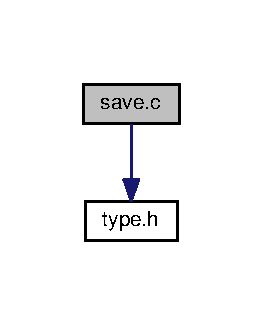
\includegraphics[width=126pt]{save_8c__incl}
\end{center}
\end{figure}
This graph shows which files directly or indirectly include this file\+:
\nopagebreak
\begin{figure}[H]
\begin{center}
\leavevmode
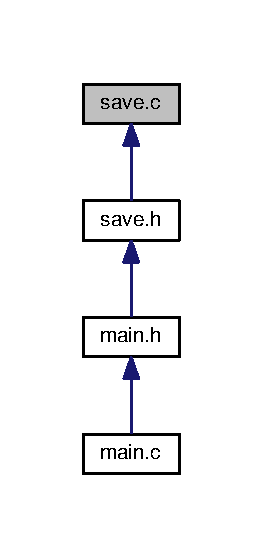
\includegraphics[width=126pt]{save_8c__dep__incl}
\end{center}
\end{figure}
\subsection*{Functions}
\begin{DoxyCompactItemize}
\item 
void {\bfseries save} (\hyperlink{structPersonne}{Personne} player, \hyperlink{structbackground}{background} map, char nom\+Fich\mbox{[}$\,$\mbox{]}, \hyperlink{structenemy}{enemy} e, int Blit\+Enemy, \hyperlink{structminimap}{minimap} m, int i, int level2, \hyperlink{structtime}{Time} T)\hypertarget{save_8c_a7a24c62188ab72e630627228c6bfb006}{}\label{save_8c_a7a24c62188ab72e630627228c6bfb006}

\item 
void {\bfseries load} (\hyperlink{structPersonne}{Personne} $\ast$player, \hyperlink{structbackground}{background} $\ast$map, char nom\+Fich\mbox{[}$\,$\mbox{]}, \hyperlink{structenemy}{enemy} $\ast$e, int $\ast$Blit\+Enemy, \hyperlink{structminimap}{minimap} $\ast$m, int $\ast$i, int $\ast$level2, \hyperlink{structtime}{Time} $\ast$T)\hypertarget{save_8c_a49d85b106316cf5001c1b22890309c17}{}\label{save_8c_a49d85b106316cf5001c1b22890309c17}

\end{DoxyCompactItemize}

%--- End generated contents ---

% Index
\backmatter
\newpage
\phantomsection
\clearemptydoublepage
\addcontentsline{toc}{chapter}{Index}
\printindex

\end{document}
